 
\documentclass{article}

\usepackage{charter}
\usepackage[english]{babel}                   % English language/hyphenation
\usepackage[protrusion=true,expansion=true]{microtype}        % Better typography
\usepackage{graphicx}                 % Enable pdflatex
%\usepackage{fix-cm}                         % Custom fontsizes
\usepackage{eurosym}                         % Euro symbol
%\usepackage[margin=3.0cm]{geometry}
\usepackage{fancyhdr}
\usepackage{lastpage} % number of last page 
\usepackage[top=2cm, bottom=4cm]{geometry}
\usepackage{hyperref}
\usepackage{pifont}% http://ctan.org/pkg/pifont
\usepackage{float} %For exact figure positioning
\usepackage{color}
\definecolor{ForestGreen}{RGB}{34,139,34}

\usepackage[table]{xcolor} 
\rowcolors{2}{gray!25}{white}


\hypersetup{
    colorlinks,
    citecolor=black,
    filecolor=black,
    linkcolor=black,
    urlcolor=black
}
\usepackage[titletoc,title]{appendix}

% Definition of \maketitle
\makeatletter         
\def\@maketitle{
\begin{center}
 FOSDEM AV Manual\\
{\Large  \@author}\\[4ex] 
\@date\\[8ex]
 
\includegraphics[width = 80mm]{logo-gear}\\

\medskip
\noindent {\Huge \bfseries \sffamily \@title }\\[4ex]
\end{center}}
\makeatother

\setcounter{tocdepth}{4}
\setcounter{secnumdepth}{4}

\title{FOSDEM AV Manual}
\author{FOSDEM Video}
\setlength{\headheight}{44pt}

\newsavebox{\LFOSDEM}
\sbox{\LFOSDEM}{
  \mbox{
    \raisebox{0pt}[4em][0pt]{
      
\includegraphics[height=3em]{logo-gear}
    }
  }
  \parbox[b]{7cm}{
    \small{
      FOSDEM AV Manual\newline
      Version: \today{}
    }
  }
}

\newsavebox{\RFOSDEM}
\sbox{\RFOSDEM}{
  \parbox[b]{4.7cm}{
    \small{
    }
  }
}

\pagestyle{fancy}
\fancyhf{}
\rhead{\usebox{\RFOSDEM}}
\lhead{\usebox{\LFOSDEM}}
\lfoot{Version: \today}
\rfoot{Page \thepage\ of \pageref{LastPage}}


\begin{document}

\maketitle \thispagestyle{empty}
\newpage

\tableofcontents
\newpage

\section{Organisation}
Video is a big task, so there are many people working together to make it all happen. In short, there are three (types of) teams:

\subsection{Setup and teardown teams}
At the start of the event/day these people take the equipment to the rooms and do basic setup (cam, sound, plugging in cables). They will ensure everything is ready before the first talk starts in each room.
At the end of the day, they will retrieve (part of) the equipment again for safe storage overnight.

During the day, they may either not be present/active or be going from room to room to fix problems, following the direction of the monitoring and control team members when needed.

\subsection{Monitoring and control team}
These people are in the NOC in the K building. They can remote into all the video boxes, and control the video part of the website.
Their task is to constantly monitor all the equipment and streams for problems, and to arrange fixes for any that occur.

There will not be enough radios for each team/room to be able to contact the central monitoring and control team, so during the setup and teardown (and possibly other busy moments), each building will have a ``control'' point (usually that buildings' service desk, if any) manned by a member of this team. Progress is kept at each local control point, which will inform the rest of the monitoring and control team through either IP (preferred) or radio (backup).

In principle, this team does not run out to fix problems themselves, but instead will sent a volunteer or similar. Maintaining contact between everyone is their main priority, and running around goes against this.

\subsection{Devroom video volunteers}
These people stay near the video equipment, keeping it safe and making sure the camera is aimed at the speaker.
They also monitor their own video/audio feeds for problems and will have means to signal problems to central control.

The devroom volunteer does not leave their post without waiting for a replacement, until the teardown team comes to collect equipment. They do \emph{NOT} disconnect or turn off any equipment themselves. That is the task of the teardown team and nobody else.

\section{FOSDEM Video Box}
The FOSDEM Video Box will take care of the streaming and recording.
There is no need to operate the controls on the camera (once on and in the correct video mode, which the setup team will have done). The setup team should also have connected the following:
\begin{itemize}
  \item At least one network cable
  \item A power cable, connected to mains, with the box already turned on
  \item Slides boxes only:
    \begin{itemize}
      \item The right jack connection should be connected to the room audio system
      \item The right VGA connection should be connected to the projector
      \item The left jack connection should have a loose mini-jack cable, for connecting to the presenter laptop
      \item The left VGA connection should have a loose VGA cable, for connecting to the presenter laptop
    \end{itemize}
  \item Cam boxes only:
    \begin{itemize}
      \item An HDMI cable to the (powered on) camera (the SDI connection is for backup and normally not in use)
    \end{itemize}
\end{itemize}

The power switch is at the back, on a standard power supply.
Order of connections and powering on does not matter, each order will work. There is no need to reboot the box after connections have changed, and there is no physical mechanism to safely power down the box.
Fully powering on the box takes about half a minute, and it will take approximately 10 seconds before anything can be seen on the LCD display. This is normal. Boot up is about twice as slow after an unexpected power loss.

\emph{Do not attempt to power off the box unassisted, as this may damage the integrity of the system.}
In the event of power loss or accidental unplugging, the system should fully auto-recover by itself. If you suspect it may be malfunctioning, first try to open the live stream yourself on any device. When problems persist, contact the control and monitoring team (see chapter ``During the event'' for full details). They may already be aware of the problem, but quick reporting helps cut down on reaction times.

While the box contains a network switch (all three ports are connected), \emph{do not connect your own equipment} to the box. The boxes are on a special subnet with reserved bandwidth for the video streaming, and any other equipment may compromise the quality of the broadcast.

\emph{The slides boxes are VGA-only.}
The internals are HDMI-compatible, but the ULD projection system only supports VGA.
Sourcing your own HDMI (and/or DP) to VGA converters is advisable, though all speakers will be informed of the VGA requirement beforehand.
The VGA signal is automatically scaled to 720p at 50Hz. Matching this on the presenter laptop is a good idea, but not a requirement.

\emph{The LCD display will inform you of all vital information about the current status of the box.} It shows a preview of the stream image (auto-refreshing screenshot, not live video), the current input resolution and refresh rate (should be 720p at 50Hz), its network status (connected/disconnected), the recording status (yes/no), the streaming status (yes/no) and audio volume level (average over the last few seconds).

The boxes report all this information to control while their network status is good, where the control and monitoring team keeps on eye on all rooms. If something is wrong, they may send somebody your way to correct it. Please follow the instructions (if any) of video team members. Keeping an eye on the box vitals and correcting any problems you notice is encouraged.

\section{Tripod}
More details coming soon.

\section{Camera}
FOSDEM2017 will use 2 different camera models: the Sony HXR-NX100 and the Canon XF100E.

\subsection{Standard settings for both cameras and quick check list}
\begin{tabular}{| l | l |}
Resolution & 1280x720 \\
Refresh rate & 50p \\
MIC-CHANNEL1(left) & Internal microphone \\
MIC-CHANNEL2(right) & Speaker microphone \\
Power source & Cable AND Battery \\
Lens cover & Remove! \\
Camera/Tripod & Cam must be attached to tripod plate \\
\end{tabular}

\subsection{Setup for Sony HXR-NX100}

\subsubsection{Screw camera on mount}
Screw the camera onto the tripod. Every camera has a screw hole at the bottom that can be used for this. The plate has a distinct ``point camera in this direction''-arrow, pay attention to this. The screw can be tightened by a coin or similar object.

\begin{figure}[H]
  \centering
  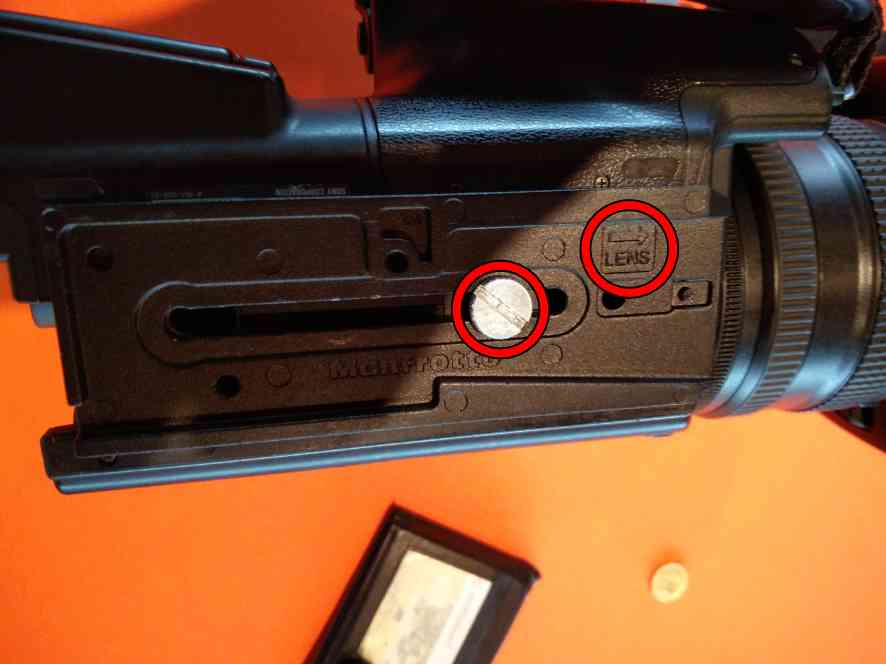
\includegraphics[width = 120mm]{Cam00.jpg}
\end{figure}

\subsubsection{Power and HDMI connectors}
First plug in the battery at the back, then plug in both the HDMI and the power cable.

Both connectors can be found next to each other to the right of the battery slot at the back.
Look at the picture if you're unsure.

Do not forget to hook up the other end of the HDMI cable to the FOSDEM Video Box, and the power cable into the mains.

\begin{figure}[H]
  \centering
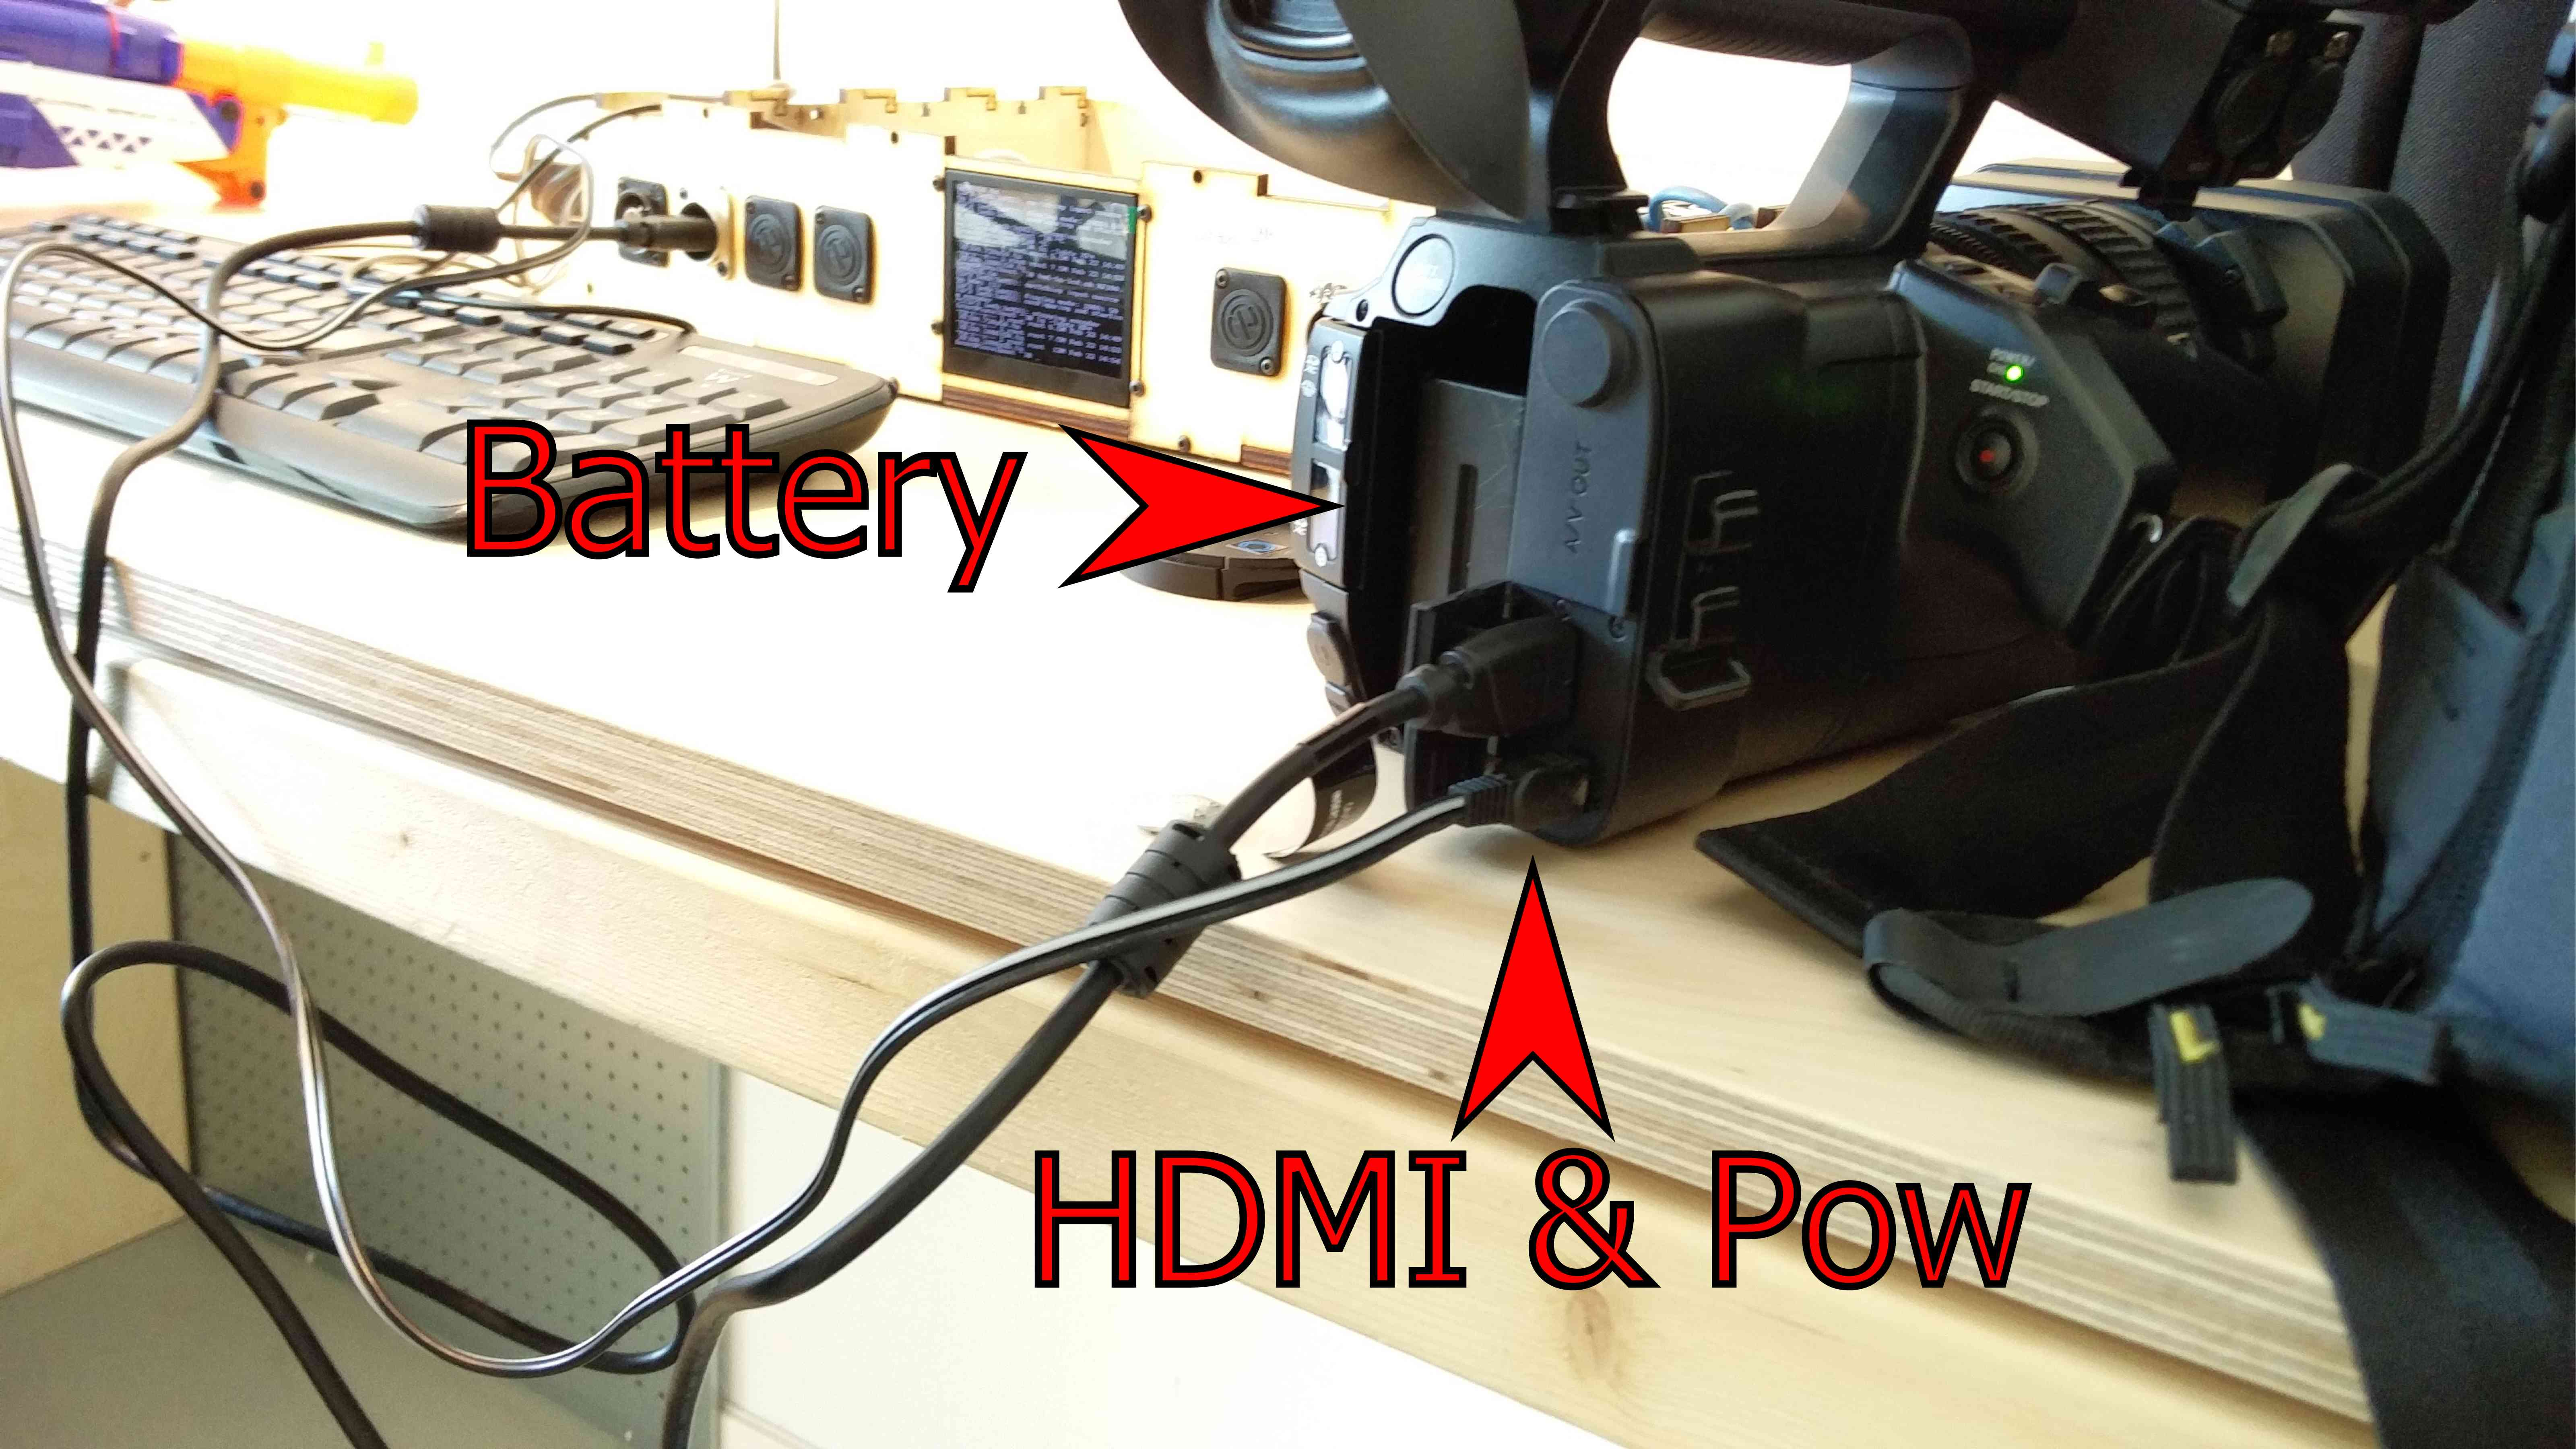
\includegraphics[width = 120mm]{Sony01.jpg}
\end{figure}

\subsubsection{Microphone}
Plug the XLR cable of the audio system into Input2.

\begin{figure}[H]
  \centering
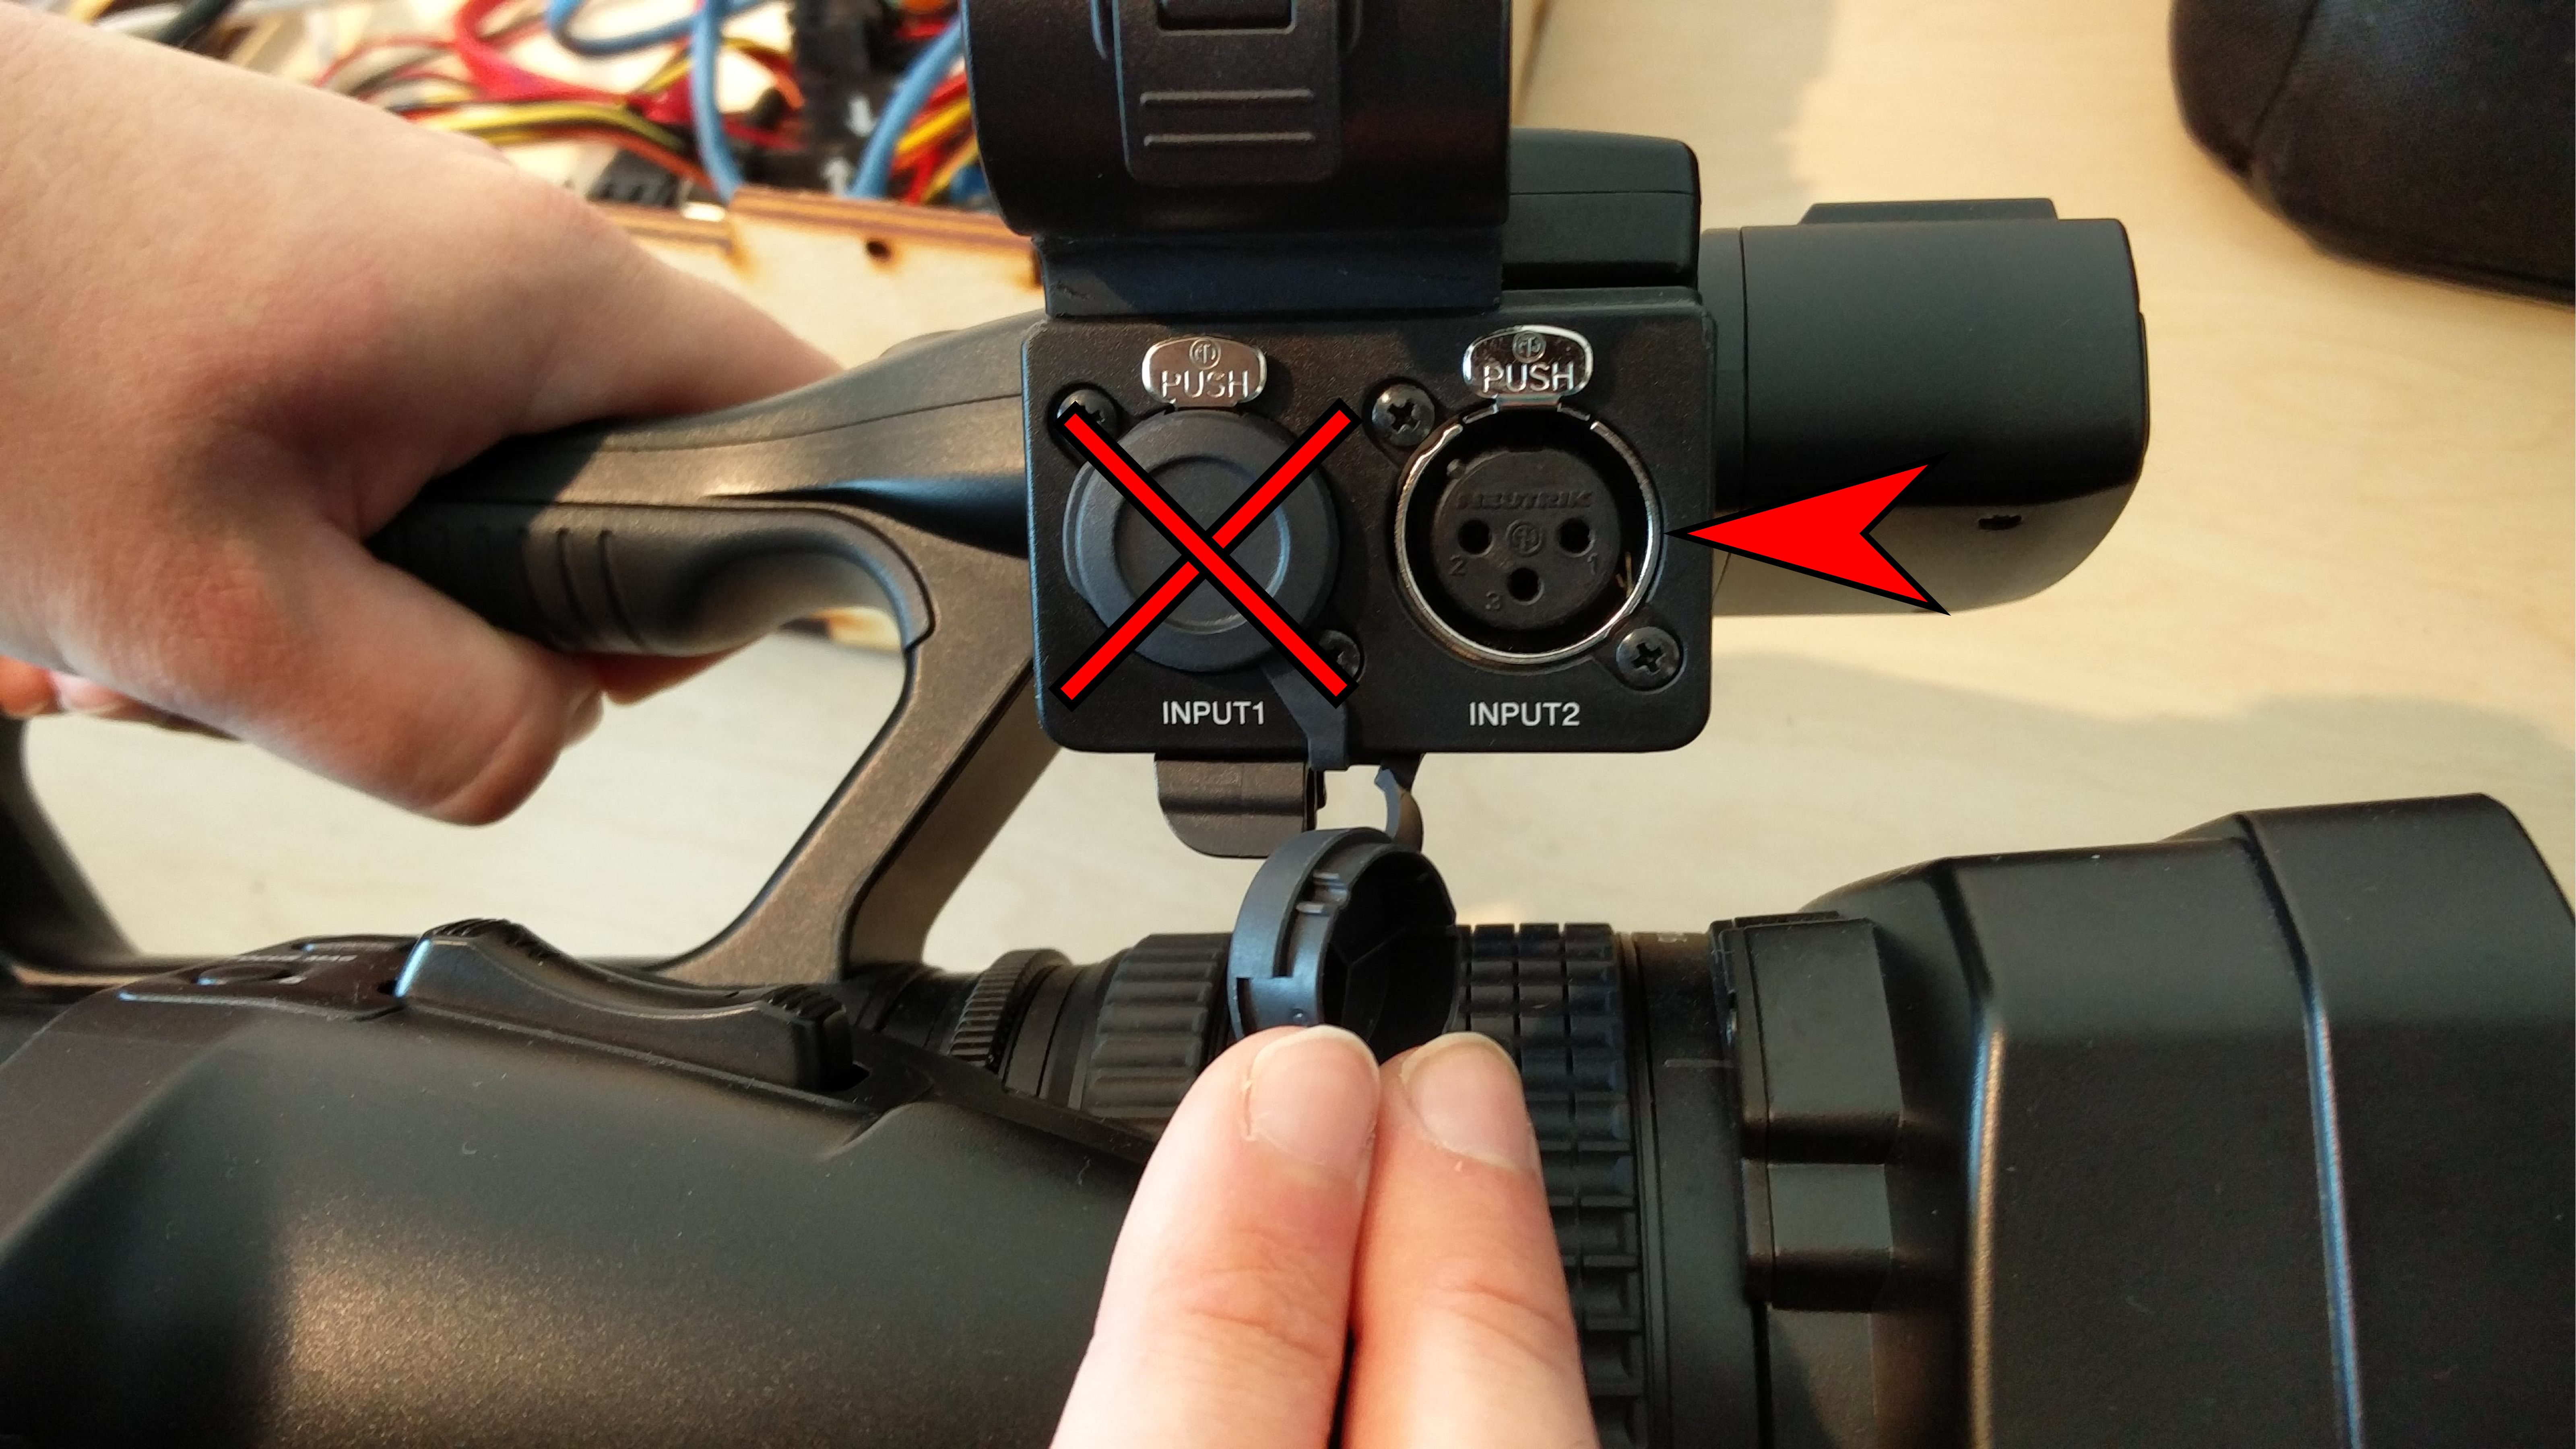
\includegraphics[width = 120mm]{Sony02.jpg}
\end{figure}

\subsubsection{Power on}
You can find the power button on the bottom of the left side of the camera (looking from behind).

\begin{figure}[H]
  \centering
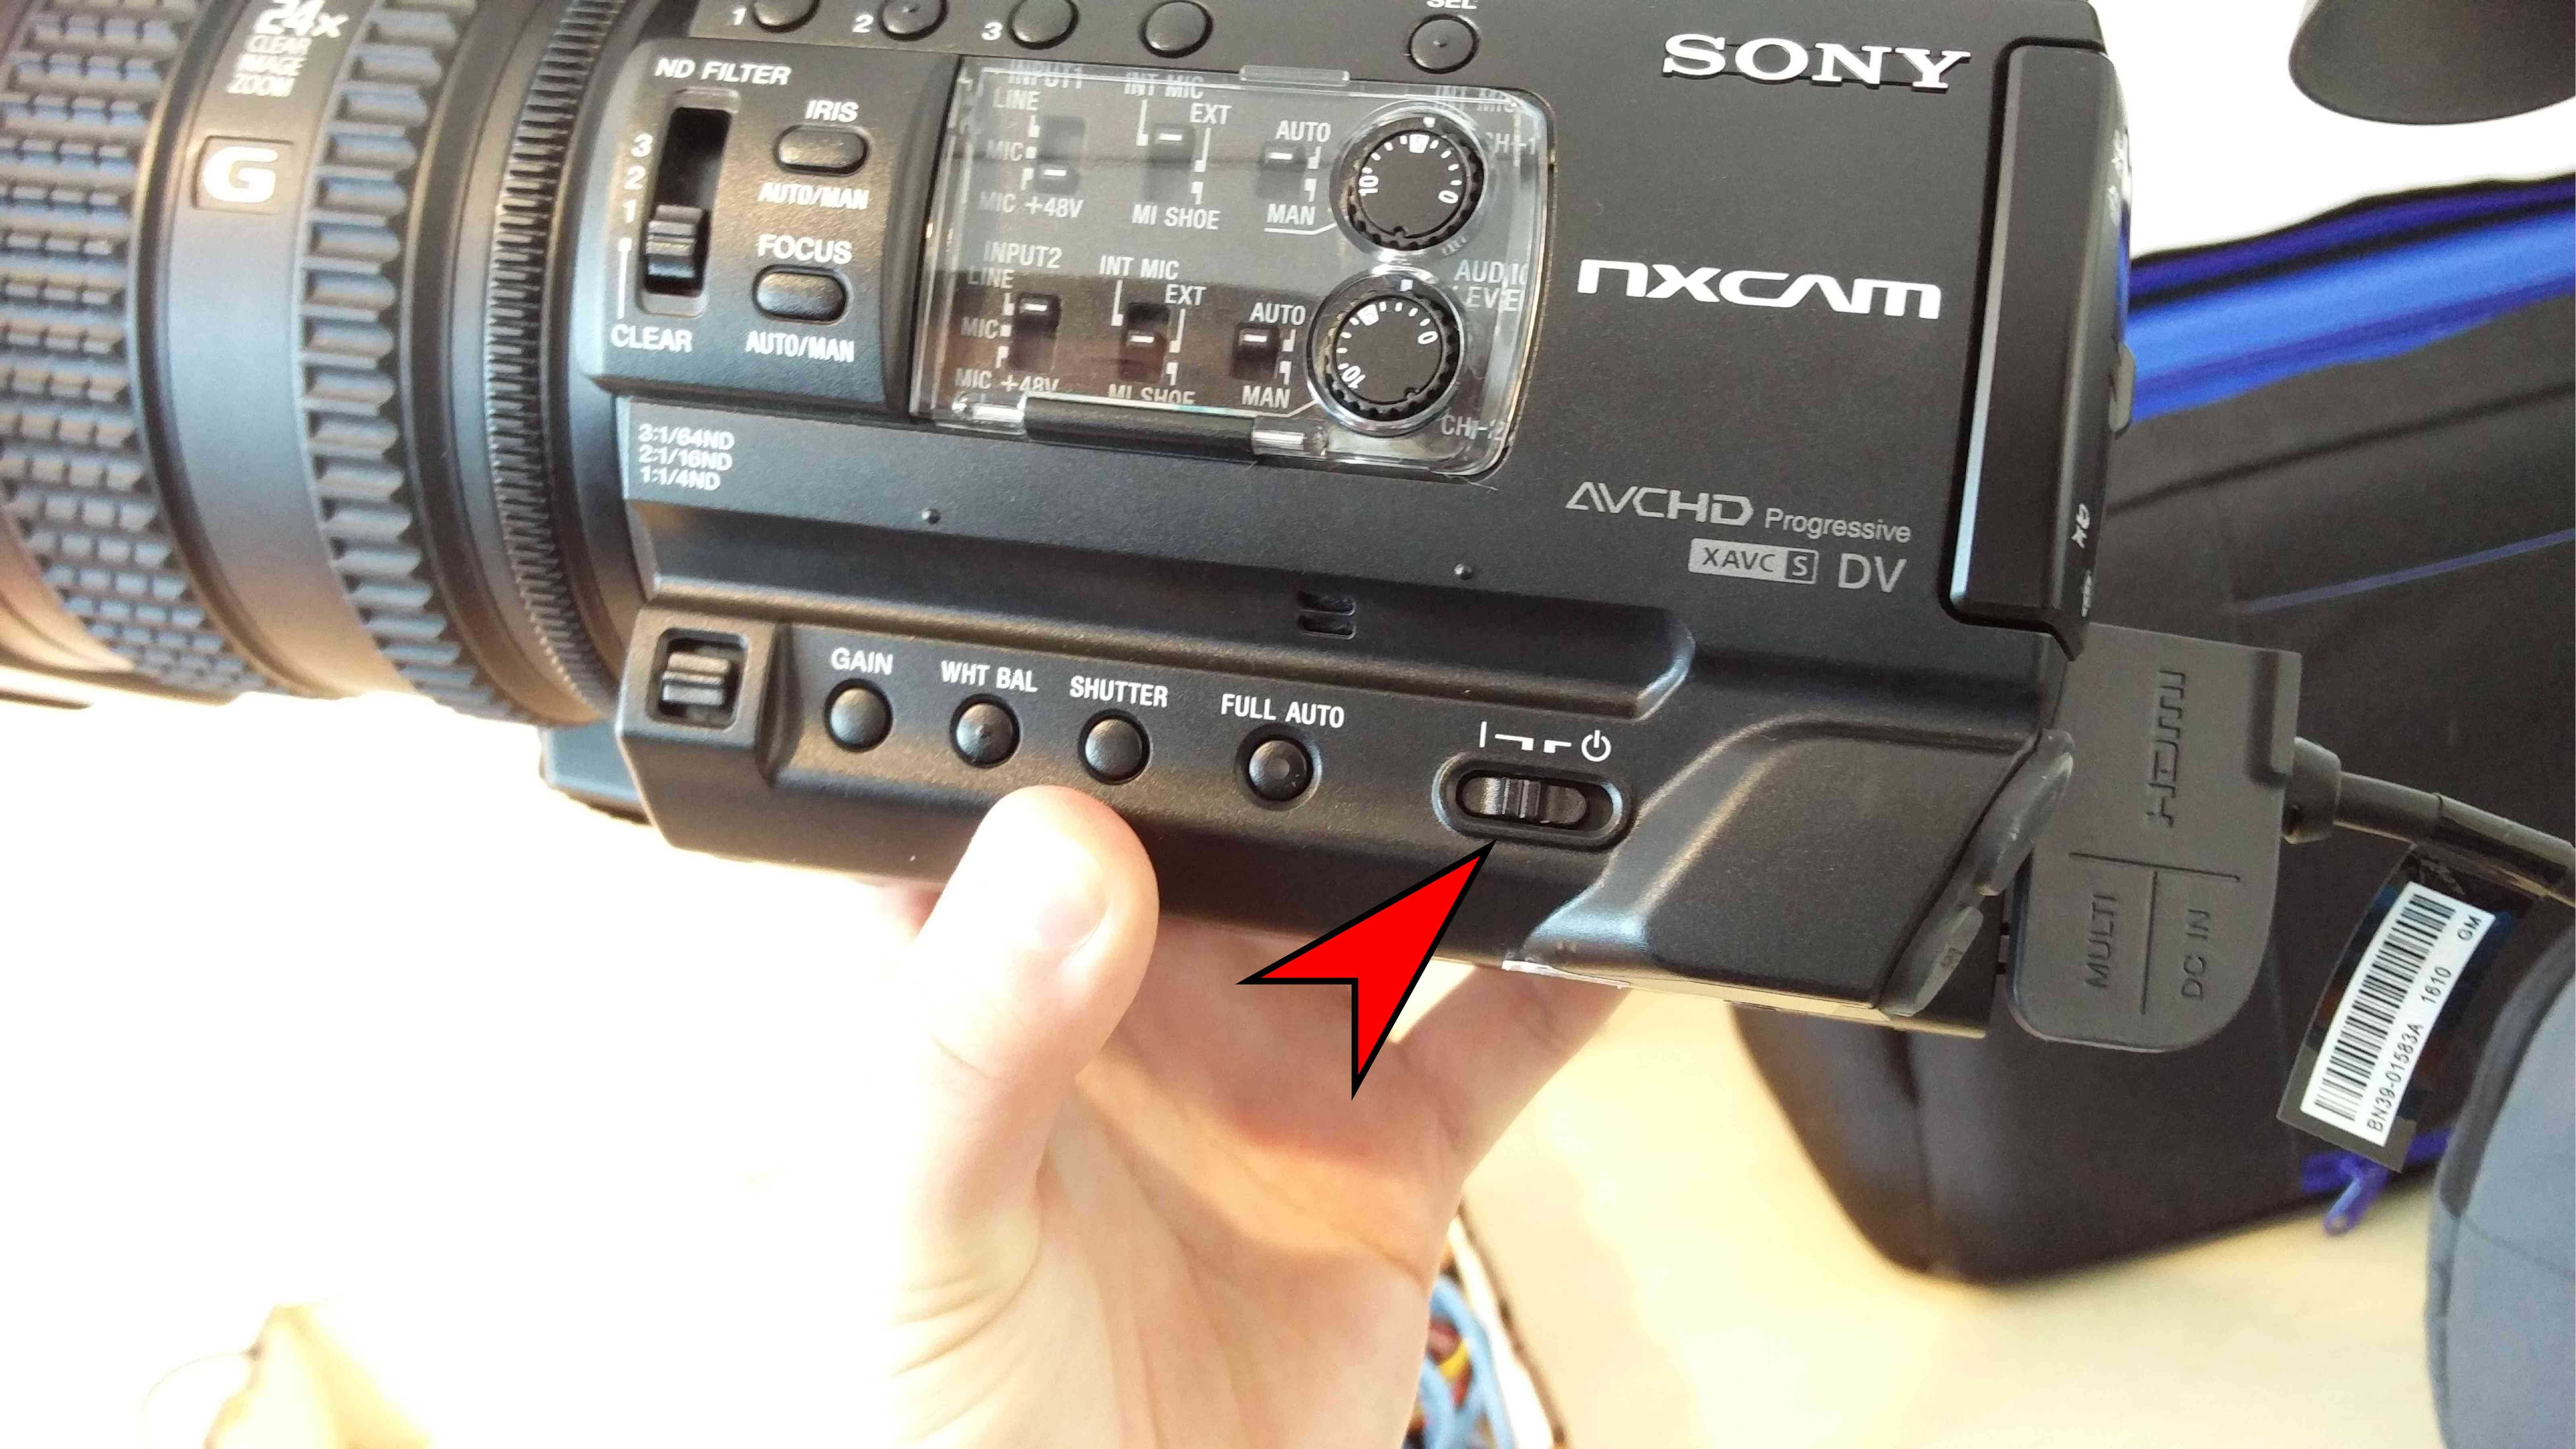
\includegraphics[width = 120mm]{Sony03.jpg}
\end{figure}

\subsubsection{Audio settings}
The audio settings can only be done through the hardware switches on the camera.
Make sure to set the switches to the correct positions, as these directly affect the availability of audio on the recordings and live streams. Wrong settings means no audio!
The position of the dials does not matter (those are for manual volume, we use automatic volume).
If unsure, verify with the image below.

\begin{tabular}{| l || l | l | l | l |}
Input & Left switch & Middle switch & Right switch & dial \\ \hline
Input1 & BOTTOM (Mic 48V) & TOP (INT MIC) & TOP (AUTO) & anything \\
Input2 & TOP (Line) & MIDDLE (EXT) & TOP (AUTO) & anything \\
\end{tabular}

\begin{figure}[H]
  \centering
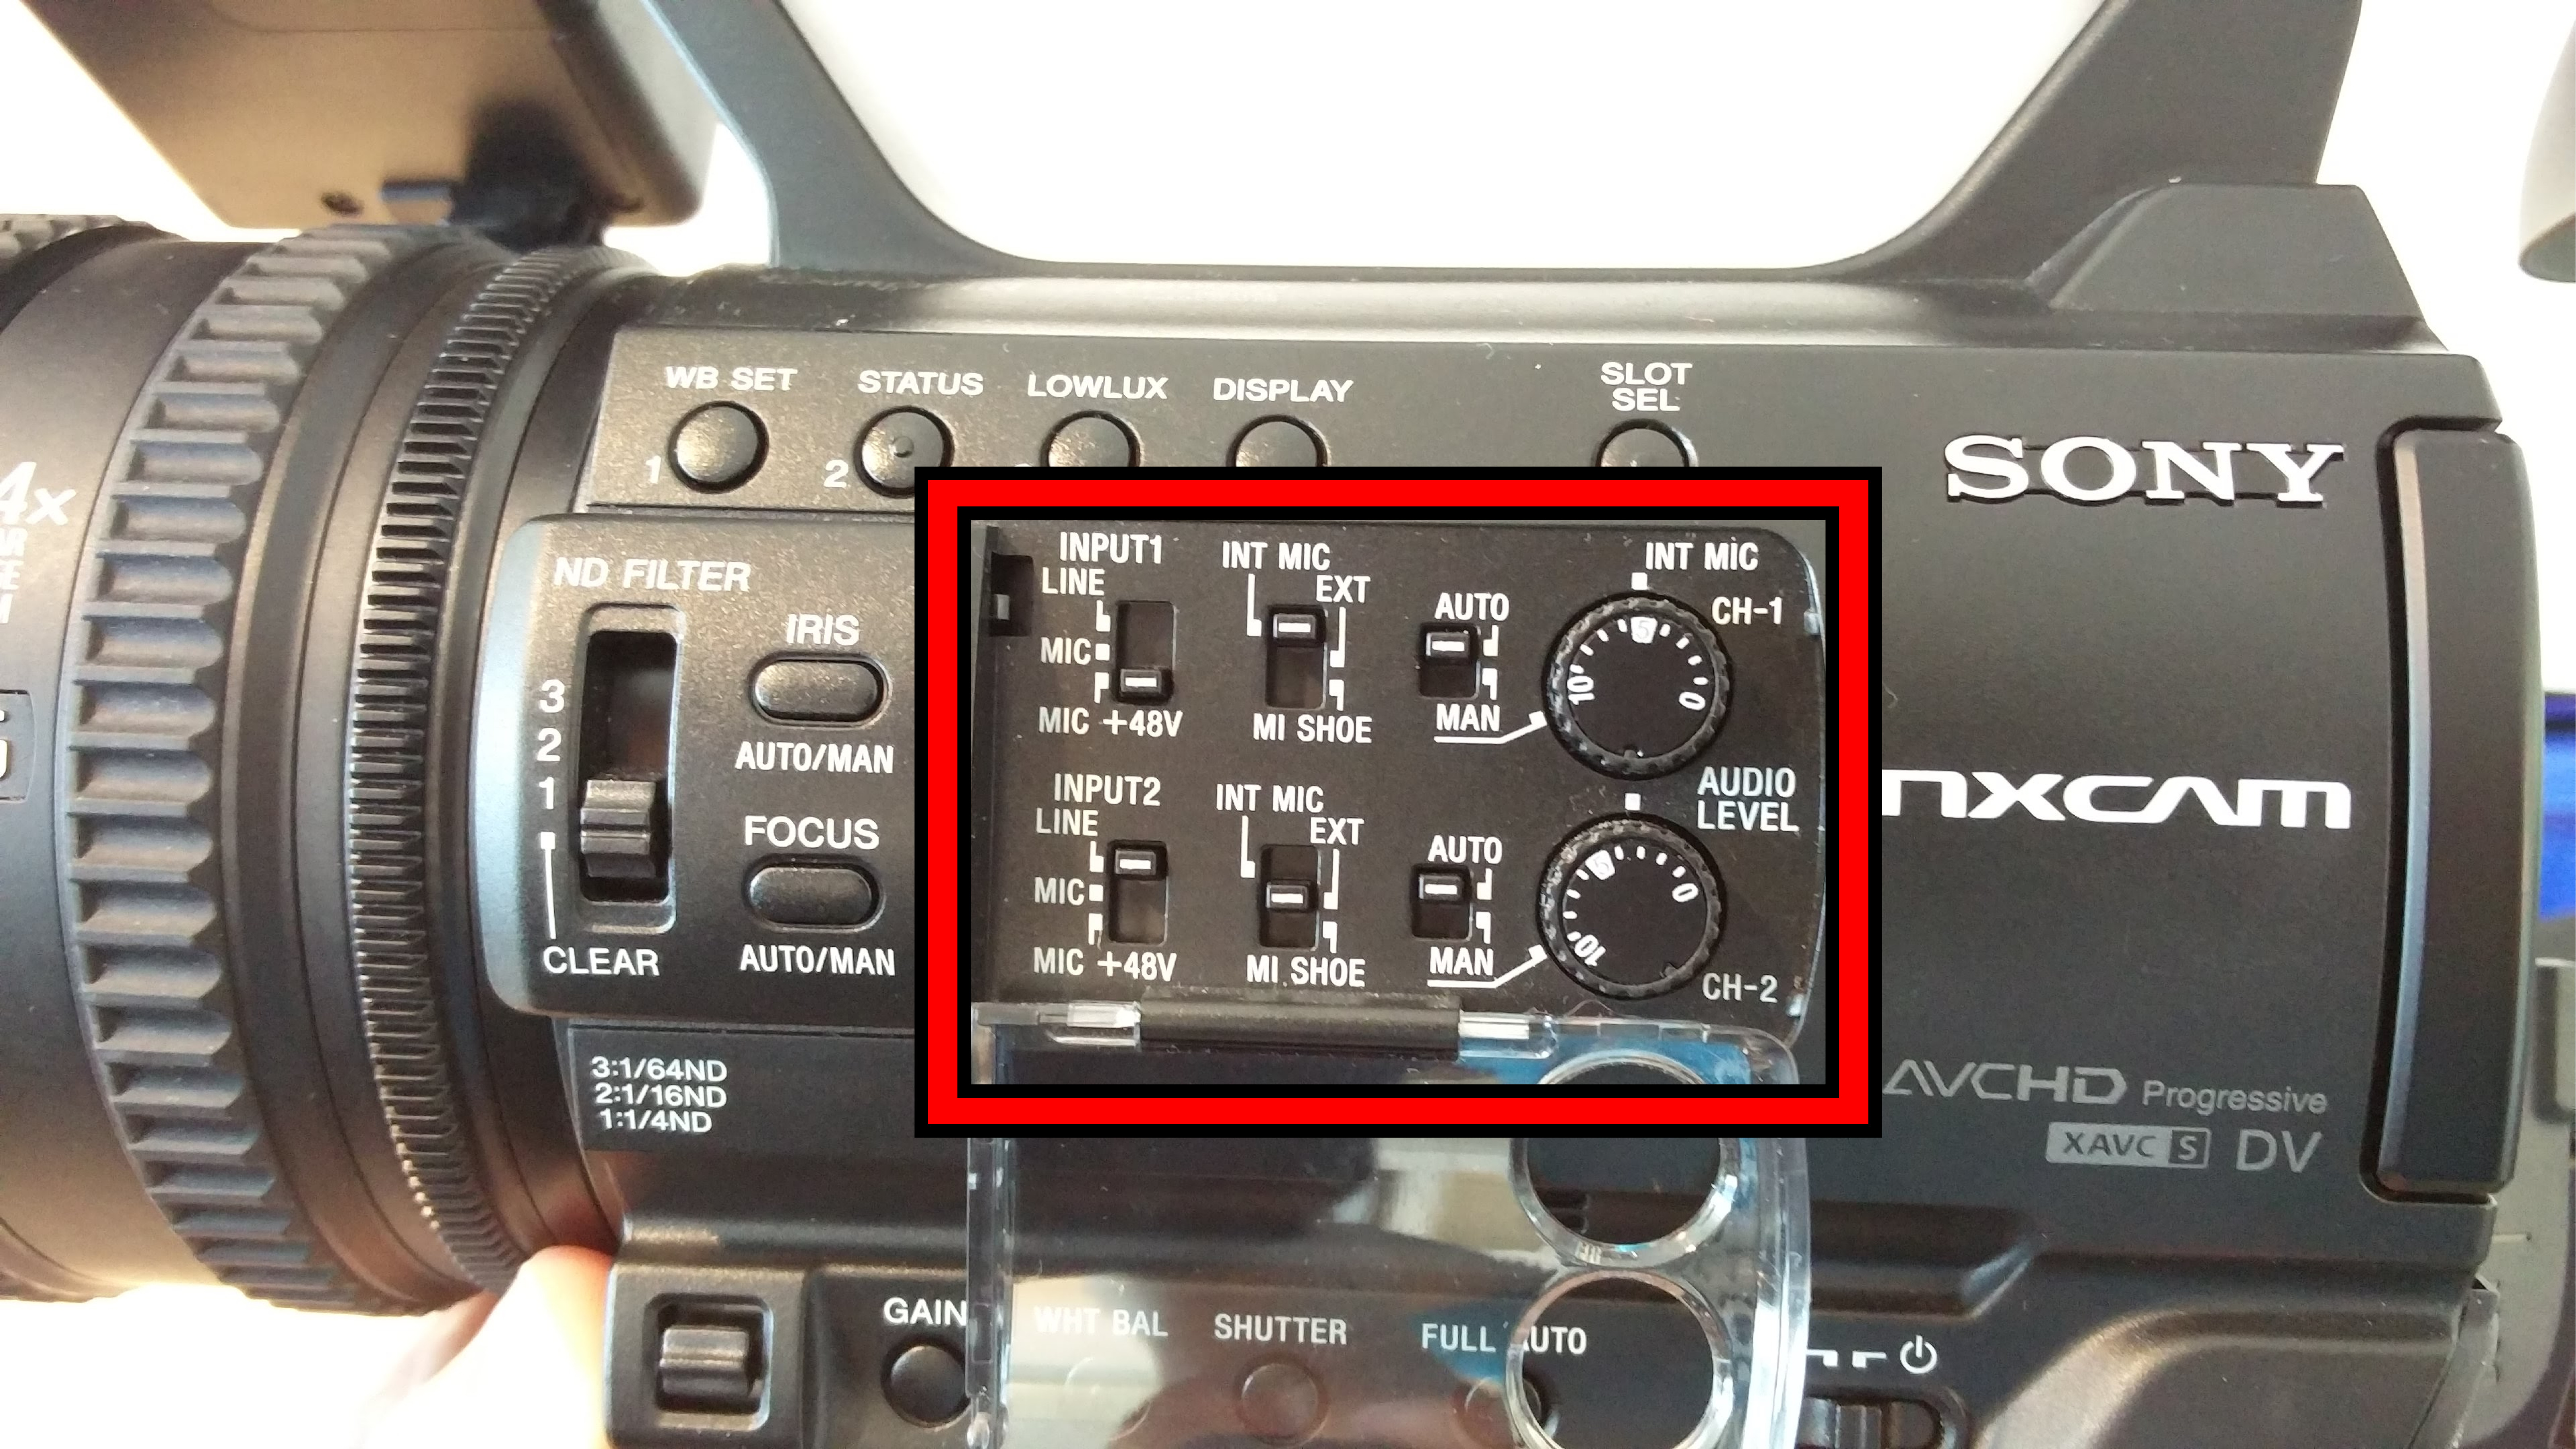
\includegraphics[width = 120mm]{Sony04.jpg}
\end{figure}

\subsubsection{Video output configuration}
The video configuration will be done through the on-screen display.

Set up like this:

Menu $\rightarrow$ 2nd icon (two arrows) $\rightarrow$ Video out $\rightarrow$ HDMI $\rightarrow$ 720p.
\begin{figure}[H]
  \centering
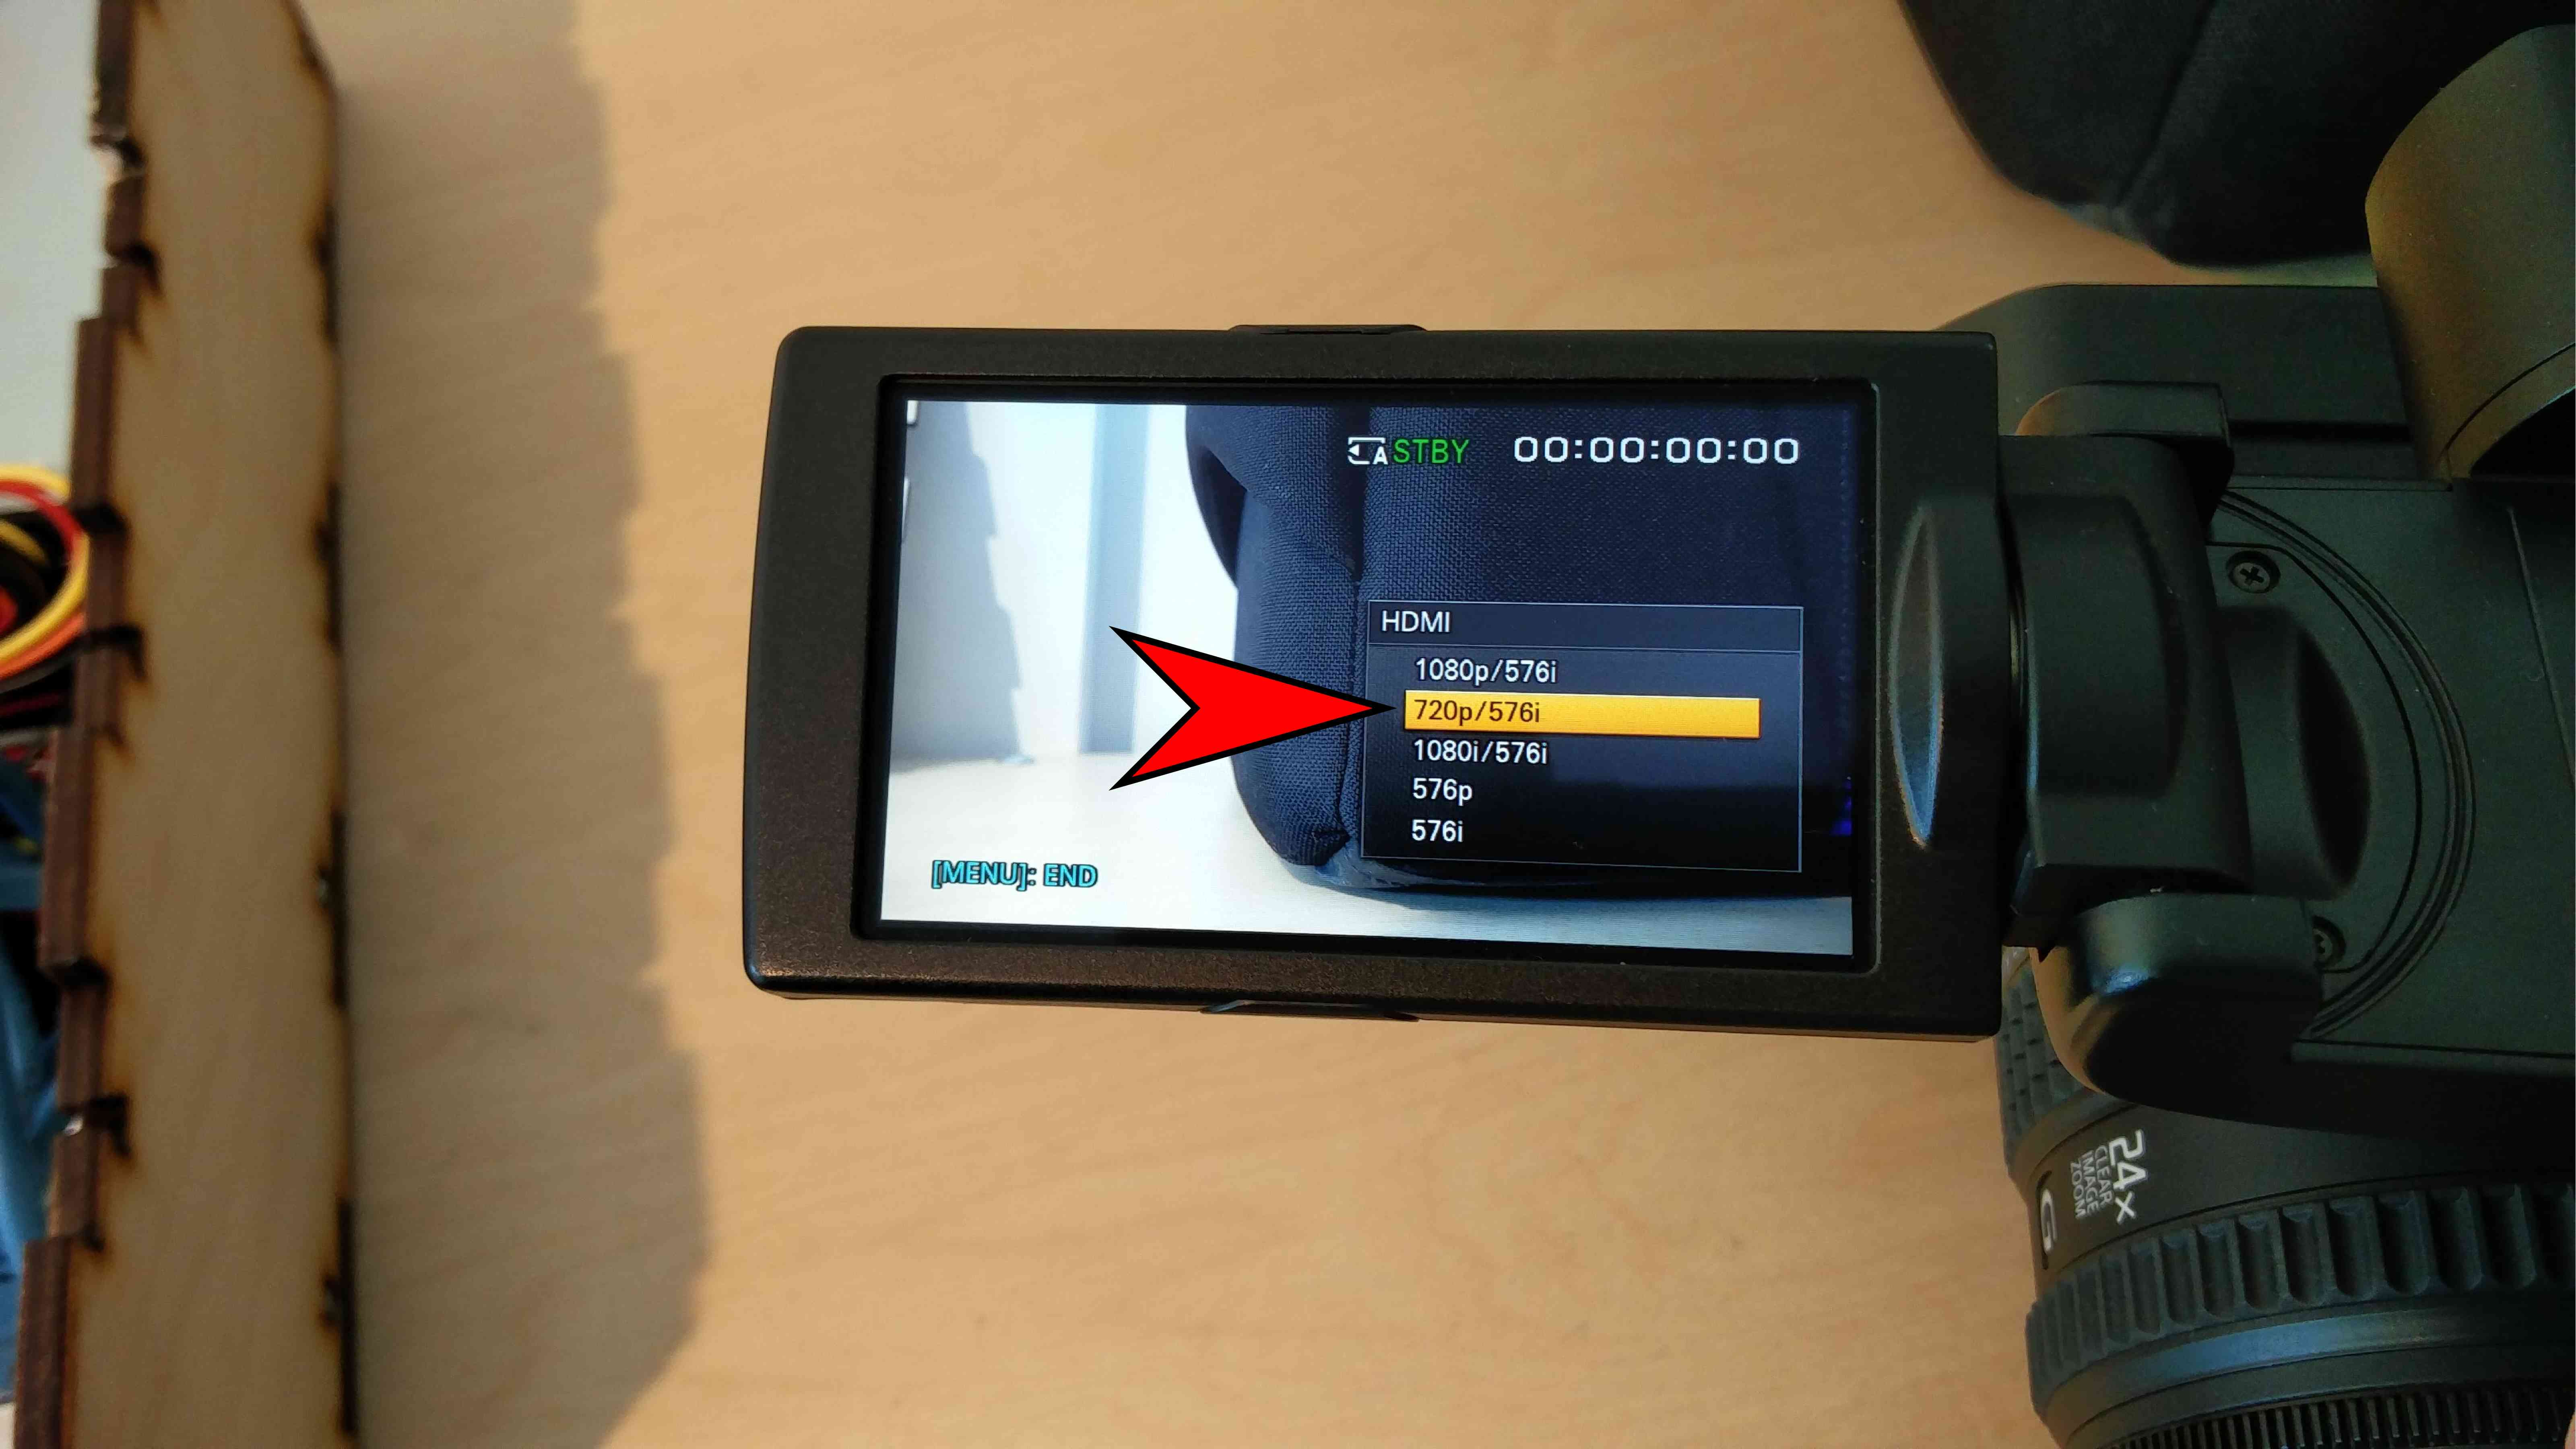
\includegraphics[width = 120mm]{Sony05.jpg}
\end{figure}

The information displayed on the OSD relates to recording to the SD card, which we do not use. \emph{Ignore this text}, as the video output config is completely separate from the recording setting on this model.
\begin{figure}[H]
  \centering
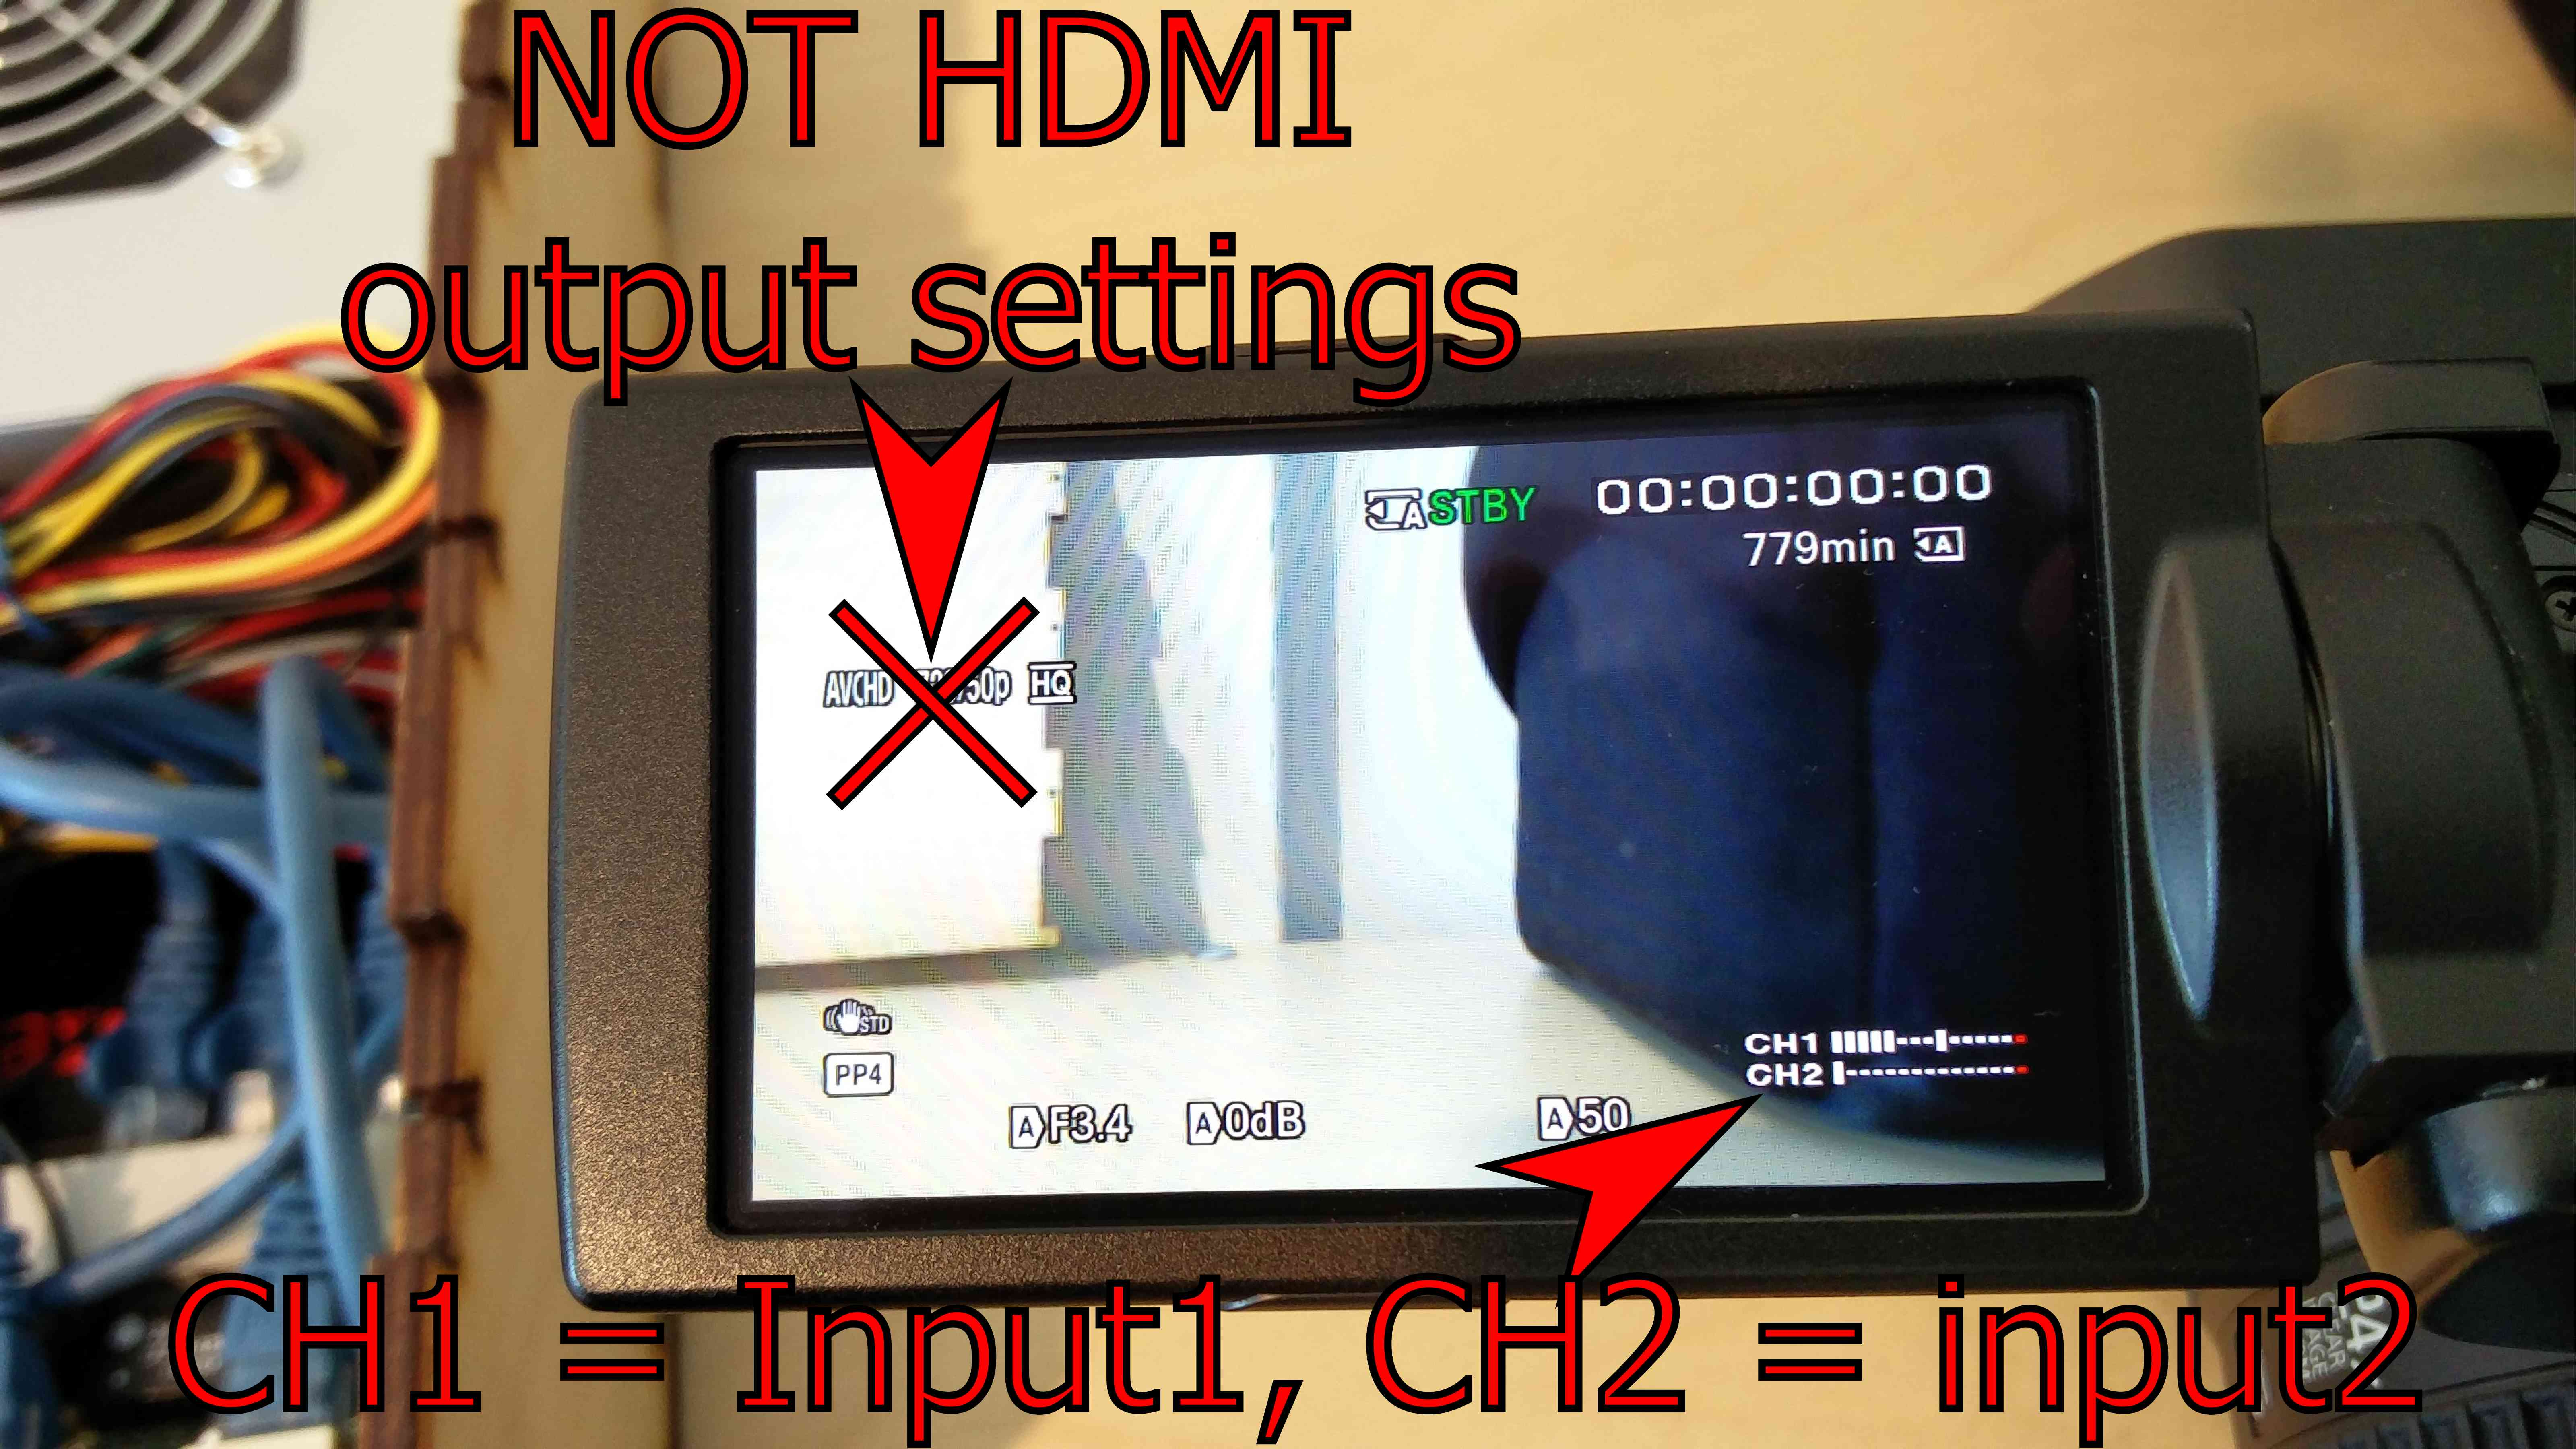
\includegraphics[width = 120mm]{Sony06.jpg}
\end{figure}

\subsubsection{Remove the lens cover}
Do not forget to remove the lens cover. Store it in the camera bag for safe keeping.

\begin{figure}[H]
  \centering
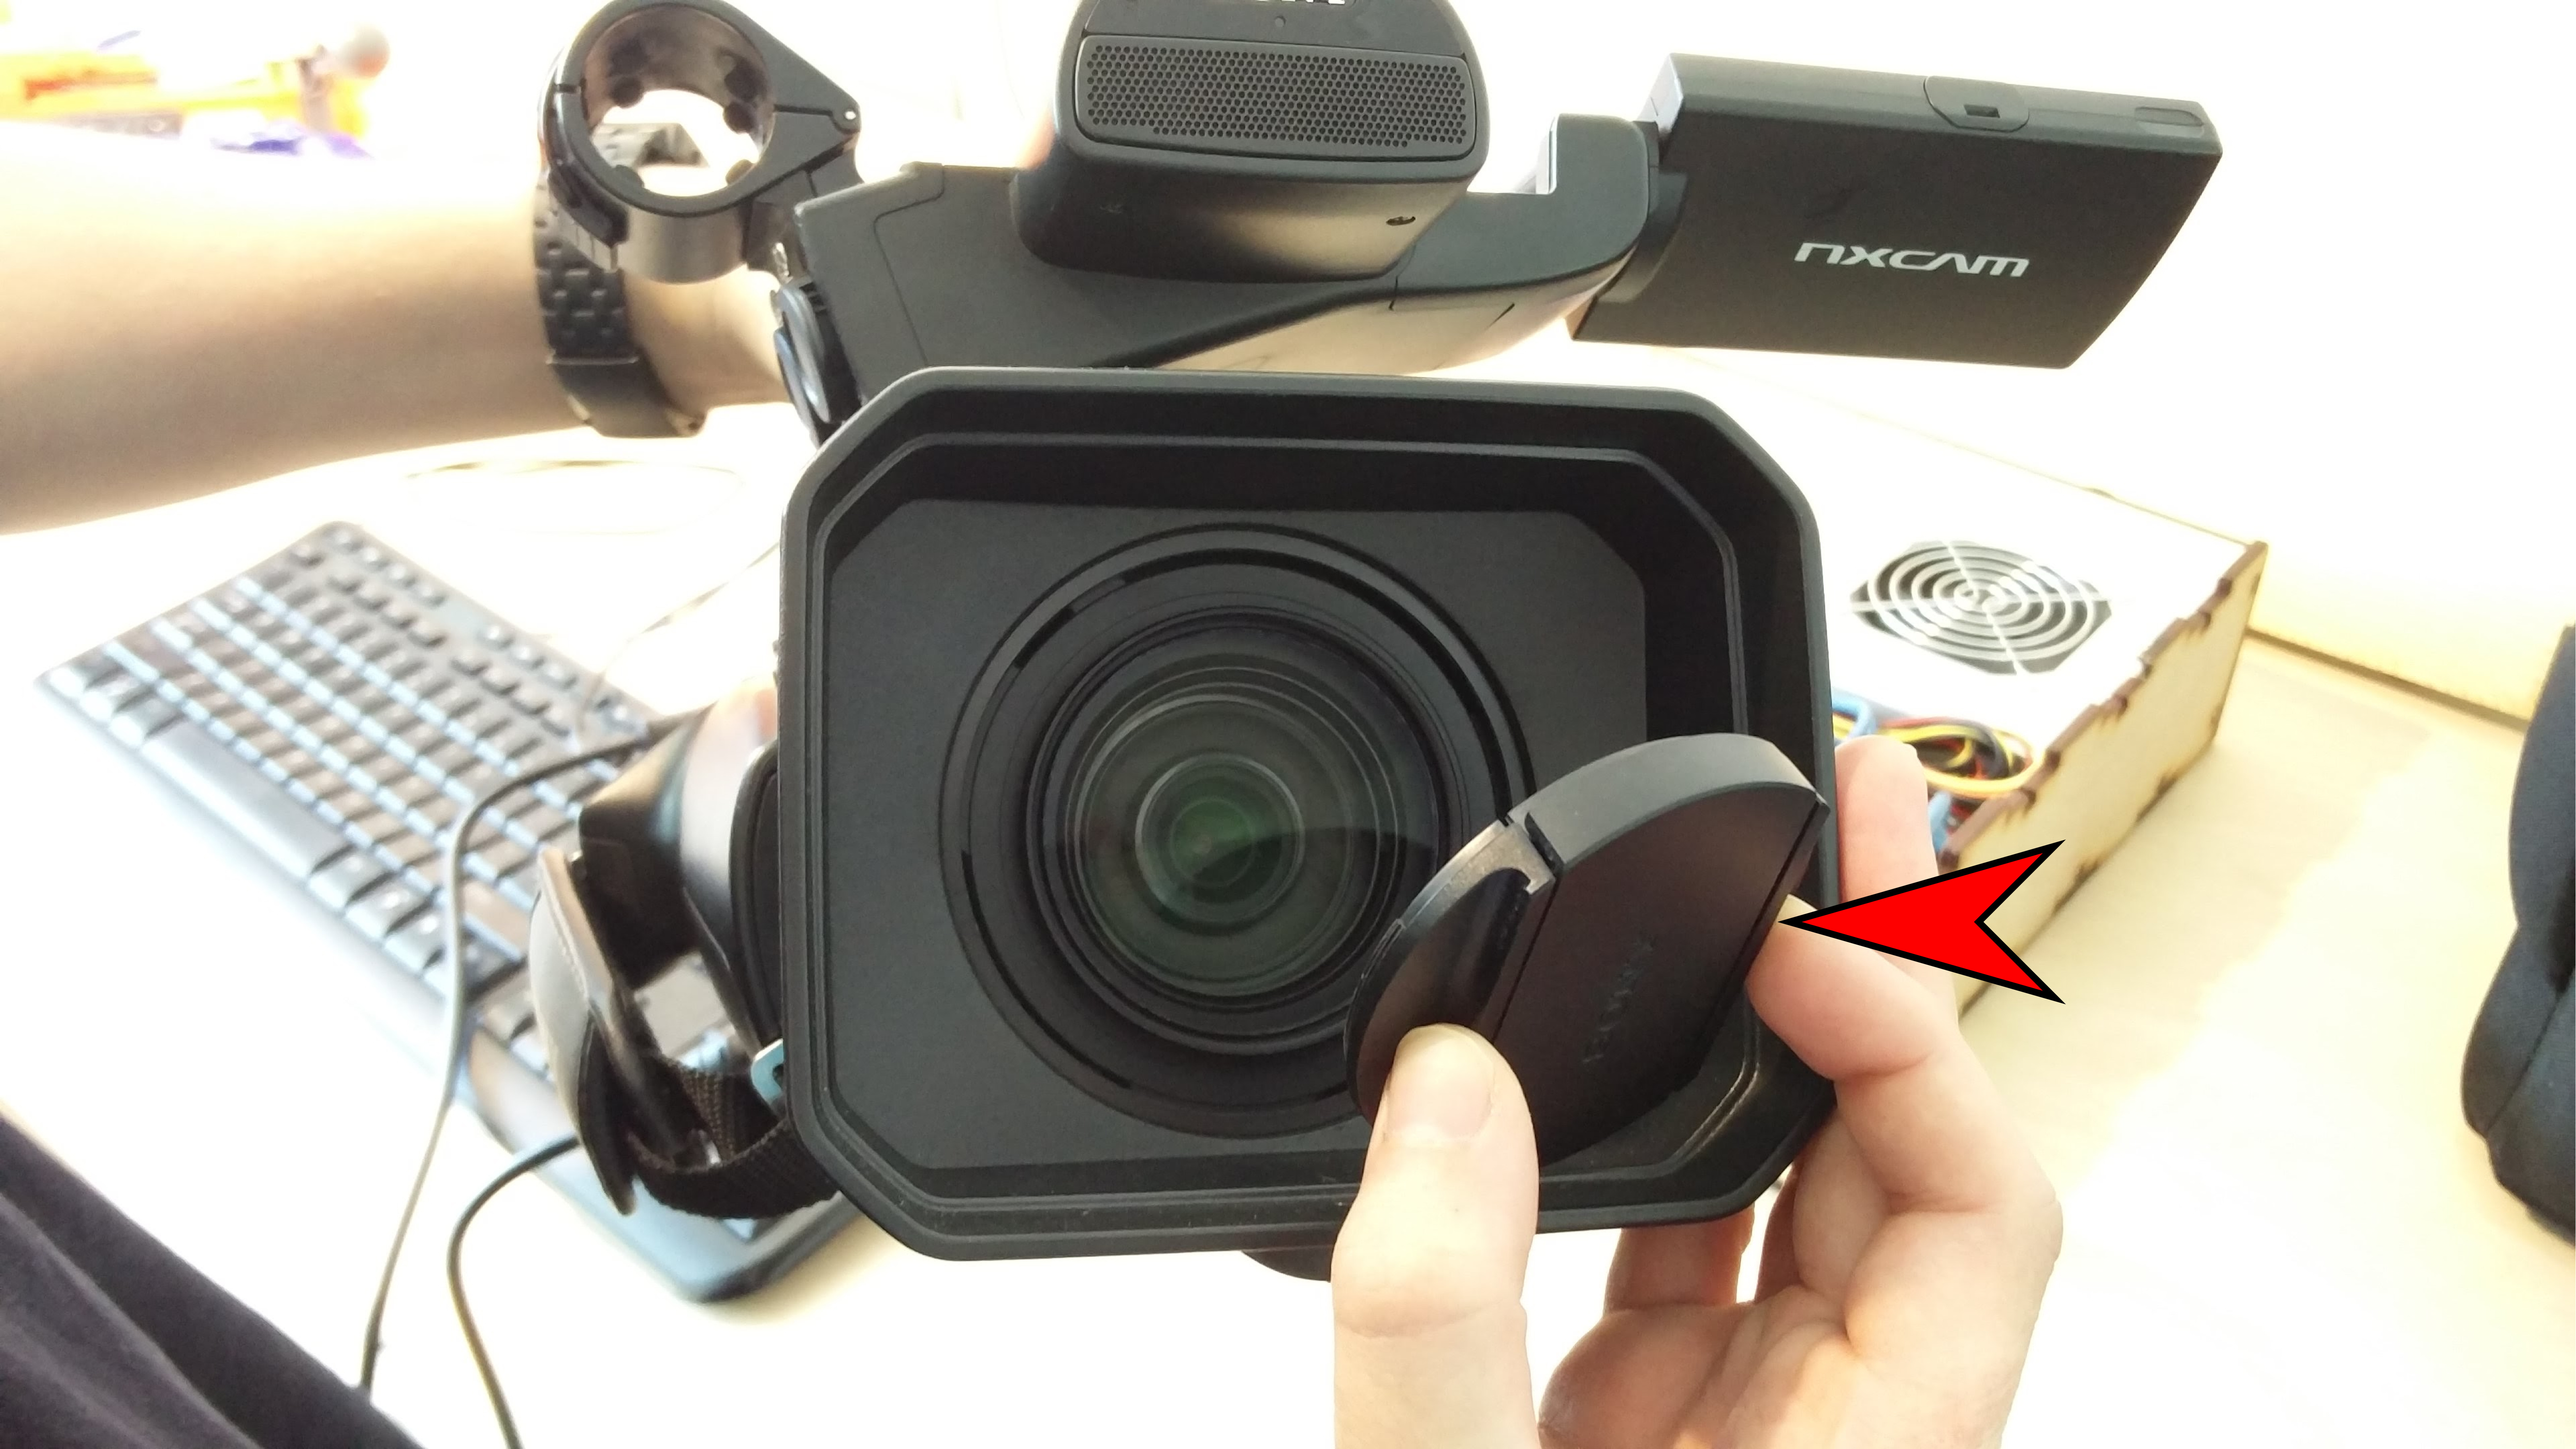
\includegraphics[width = 120mm]{Sony07.jpg}
\end{figure}

\subsubsection{Checklist}
Please check the following before leaving:
\begin{itemize}
  \item Does CH1 on the camera display spike when you tap the camera itself with your fingers?
  \item Does CH2 on the camera display spike when you tap the (powered on) wireless speaker microphone?
  \item Turn off the wireless speaker microphone before leaving to conserve battery power for during the day.
  \item Do both video boxes say mode 720p50 on the LCD display?
  \item Does the camera video box display the camera image on the LCD display?
\end{itemize}

If any of these do not work, re-check your connections and settings. Still no luck? Contract control!

\subsubsection{Contact control}
Please report that you've finished the room with your local control point.
They will let you know what rooms still need attention.

\subsection{Setup for Canon XF100E}

\subsubsection{Screw camera on mount}
Screw the camera onto the tripod. Every camera has a screw hole at the bottom that can be used for this. The plate has a distinct ``point camera in this direction''-arrow, pay attention to this. The screw can be tightened by a coin or similar object.

\begin{figure}[H]
  \centering
  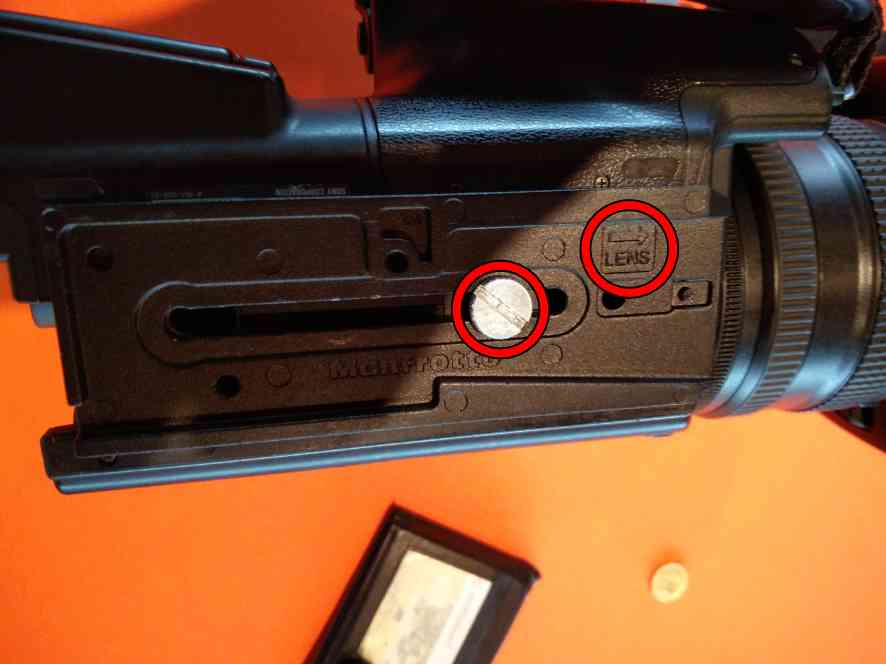
\includegraphics[width = 120mm]{Cam00.jpg}
\end{figure}


\subsubsection{Power and HDMI connectors}
First plug in the battery at the back, then plug in both the HDMI and the power cable.

The HDMI connector is hidden behind a cover on the bottom of the right side.
Power is on the back, to the left of the battery slot.
Look at the picture if you're unsure.

Do not forget to hook up the other end of the HDMI cable to the FOSDEM Video Box, and the power cable into the mains.

\begin{figure}[H]
  \centering
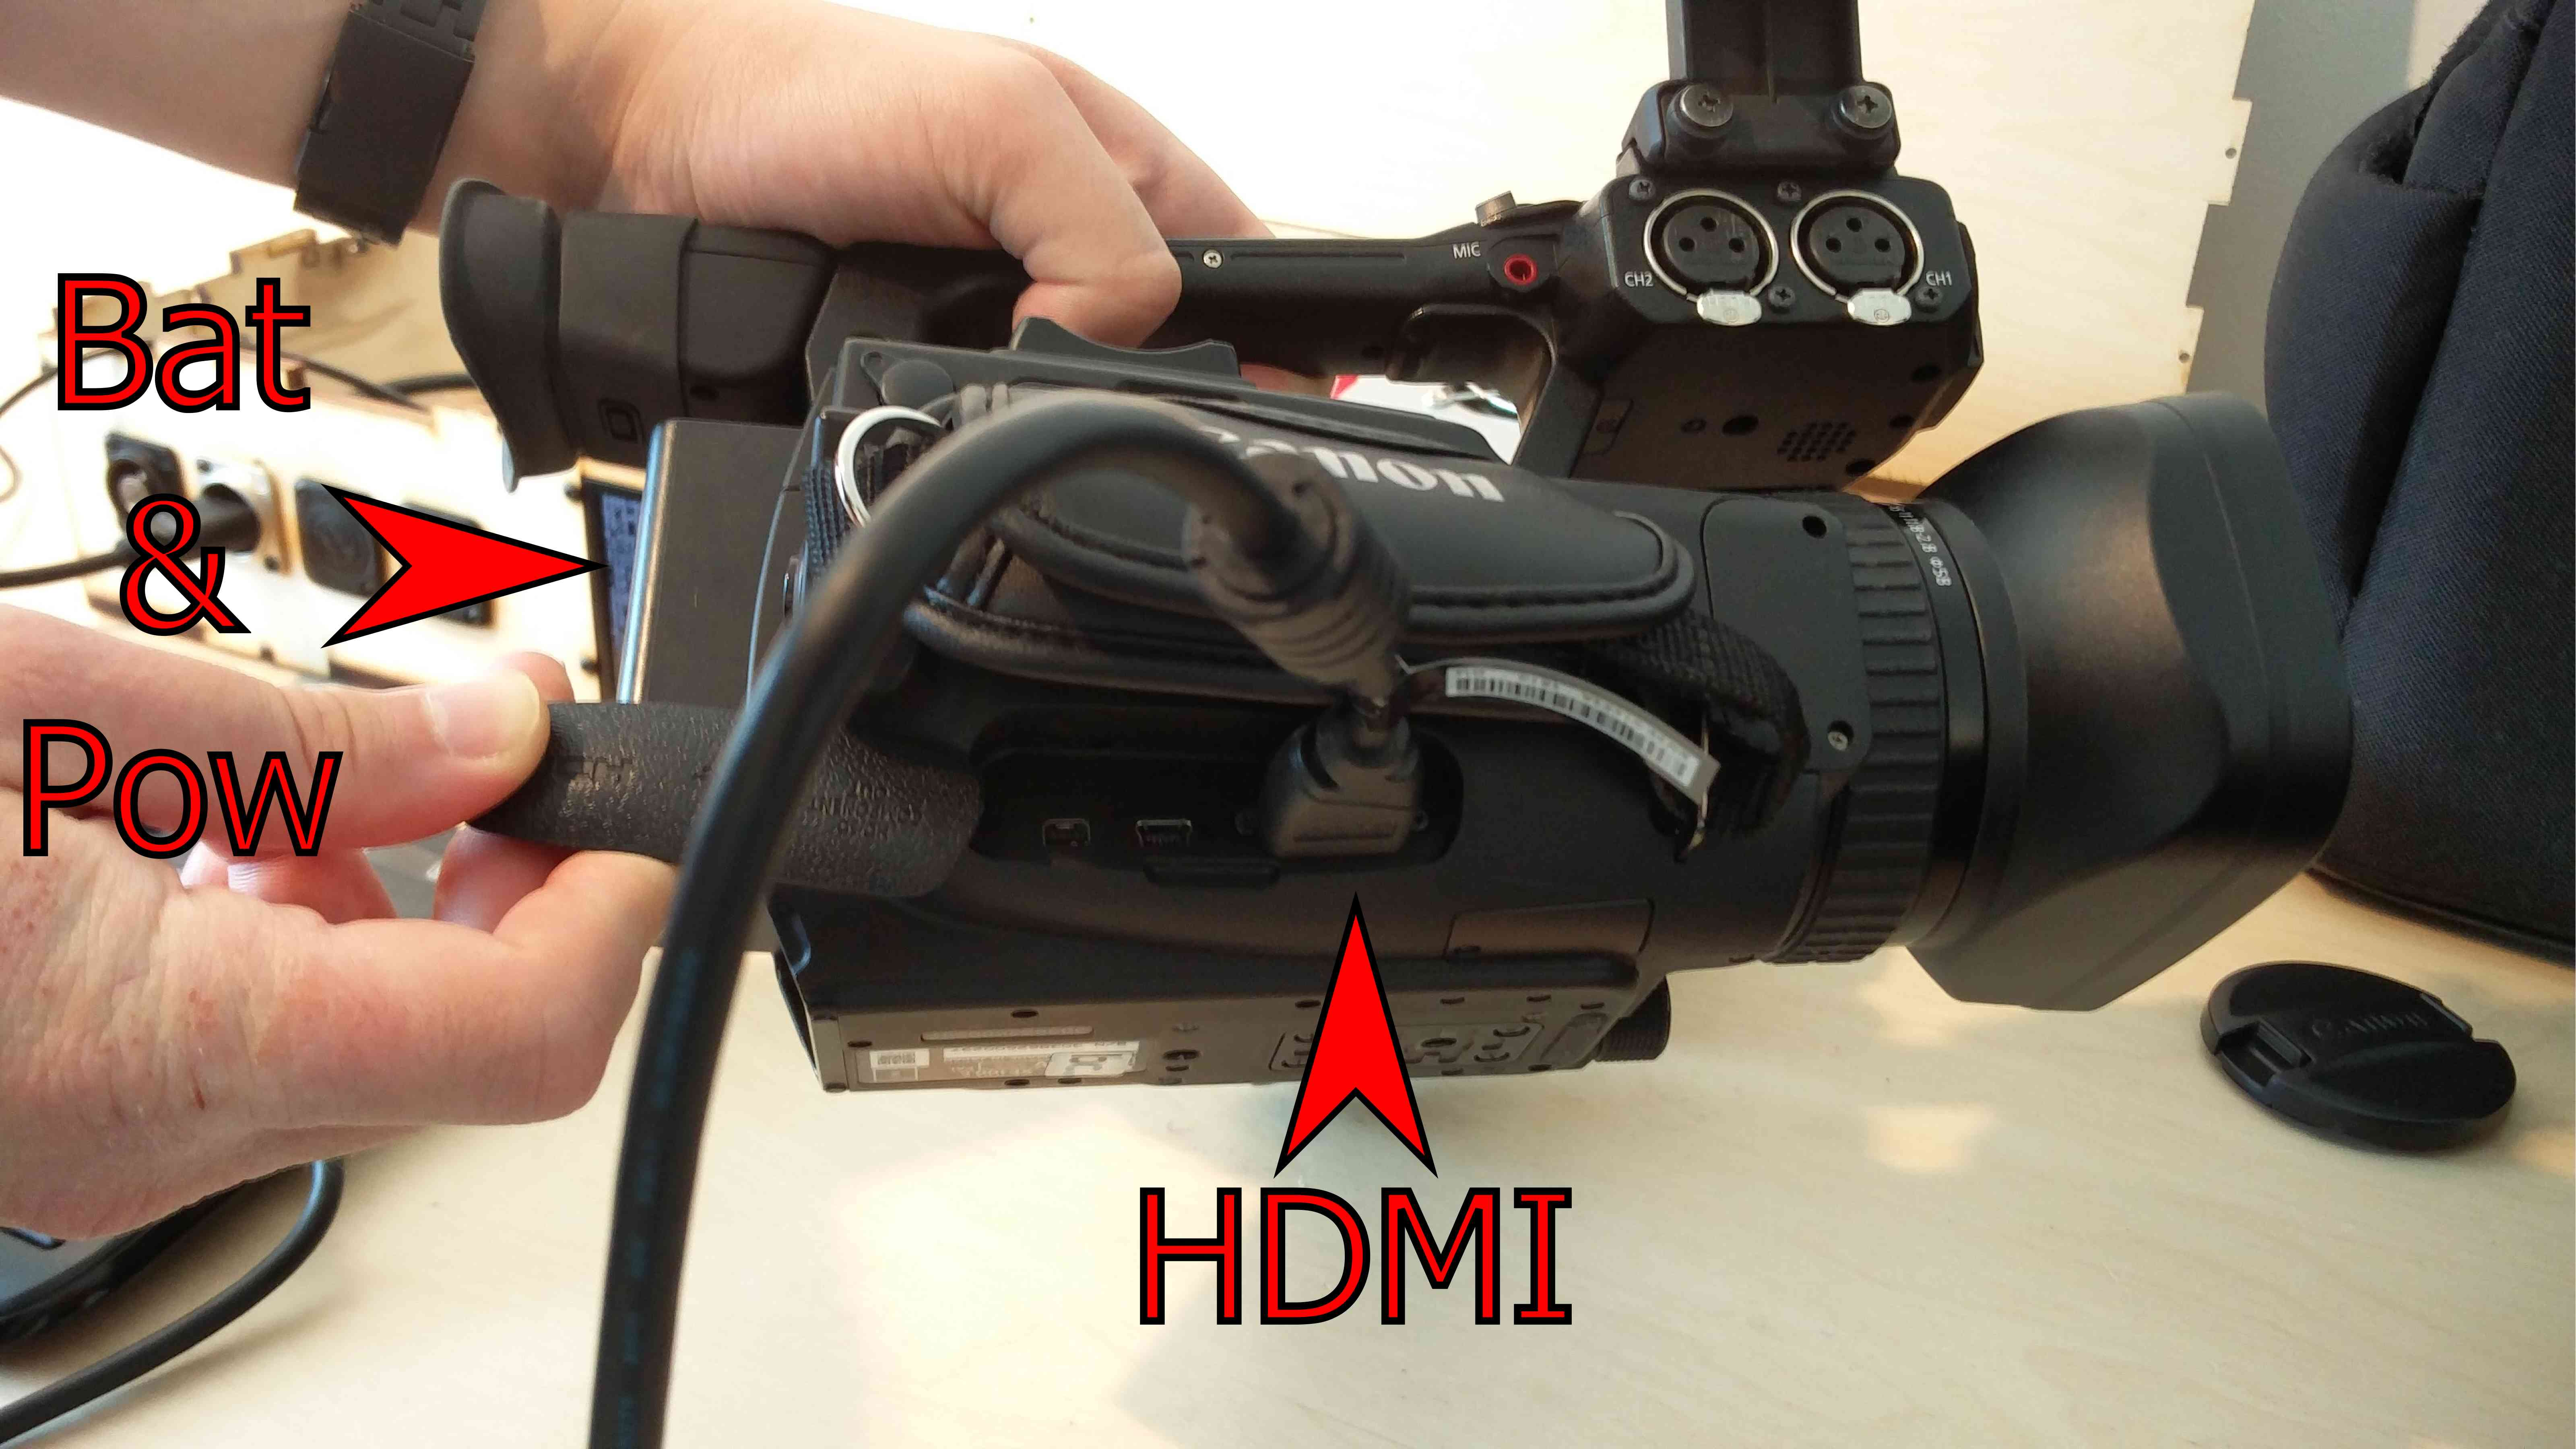
\includegraphics[width = 120mm]{Canon01.jpg}
\end{figure}

\subsubsection{Microphone}
Plug the XLR cable of the audio system into CH2.

\begin{figure}[H]
  \centering
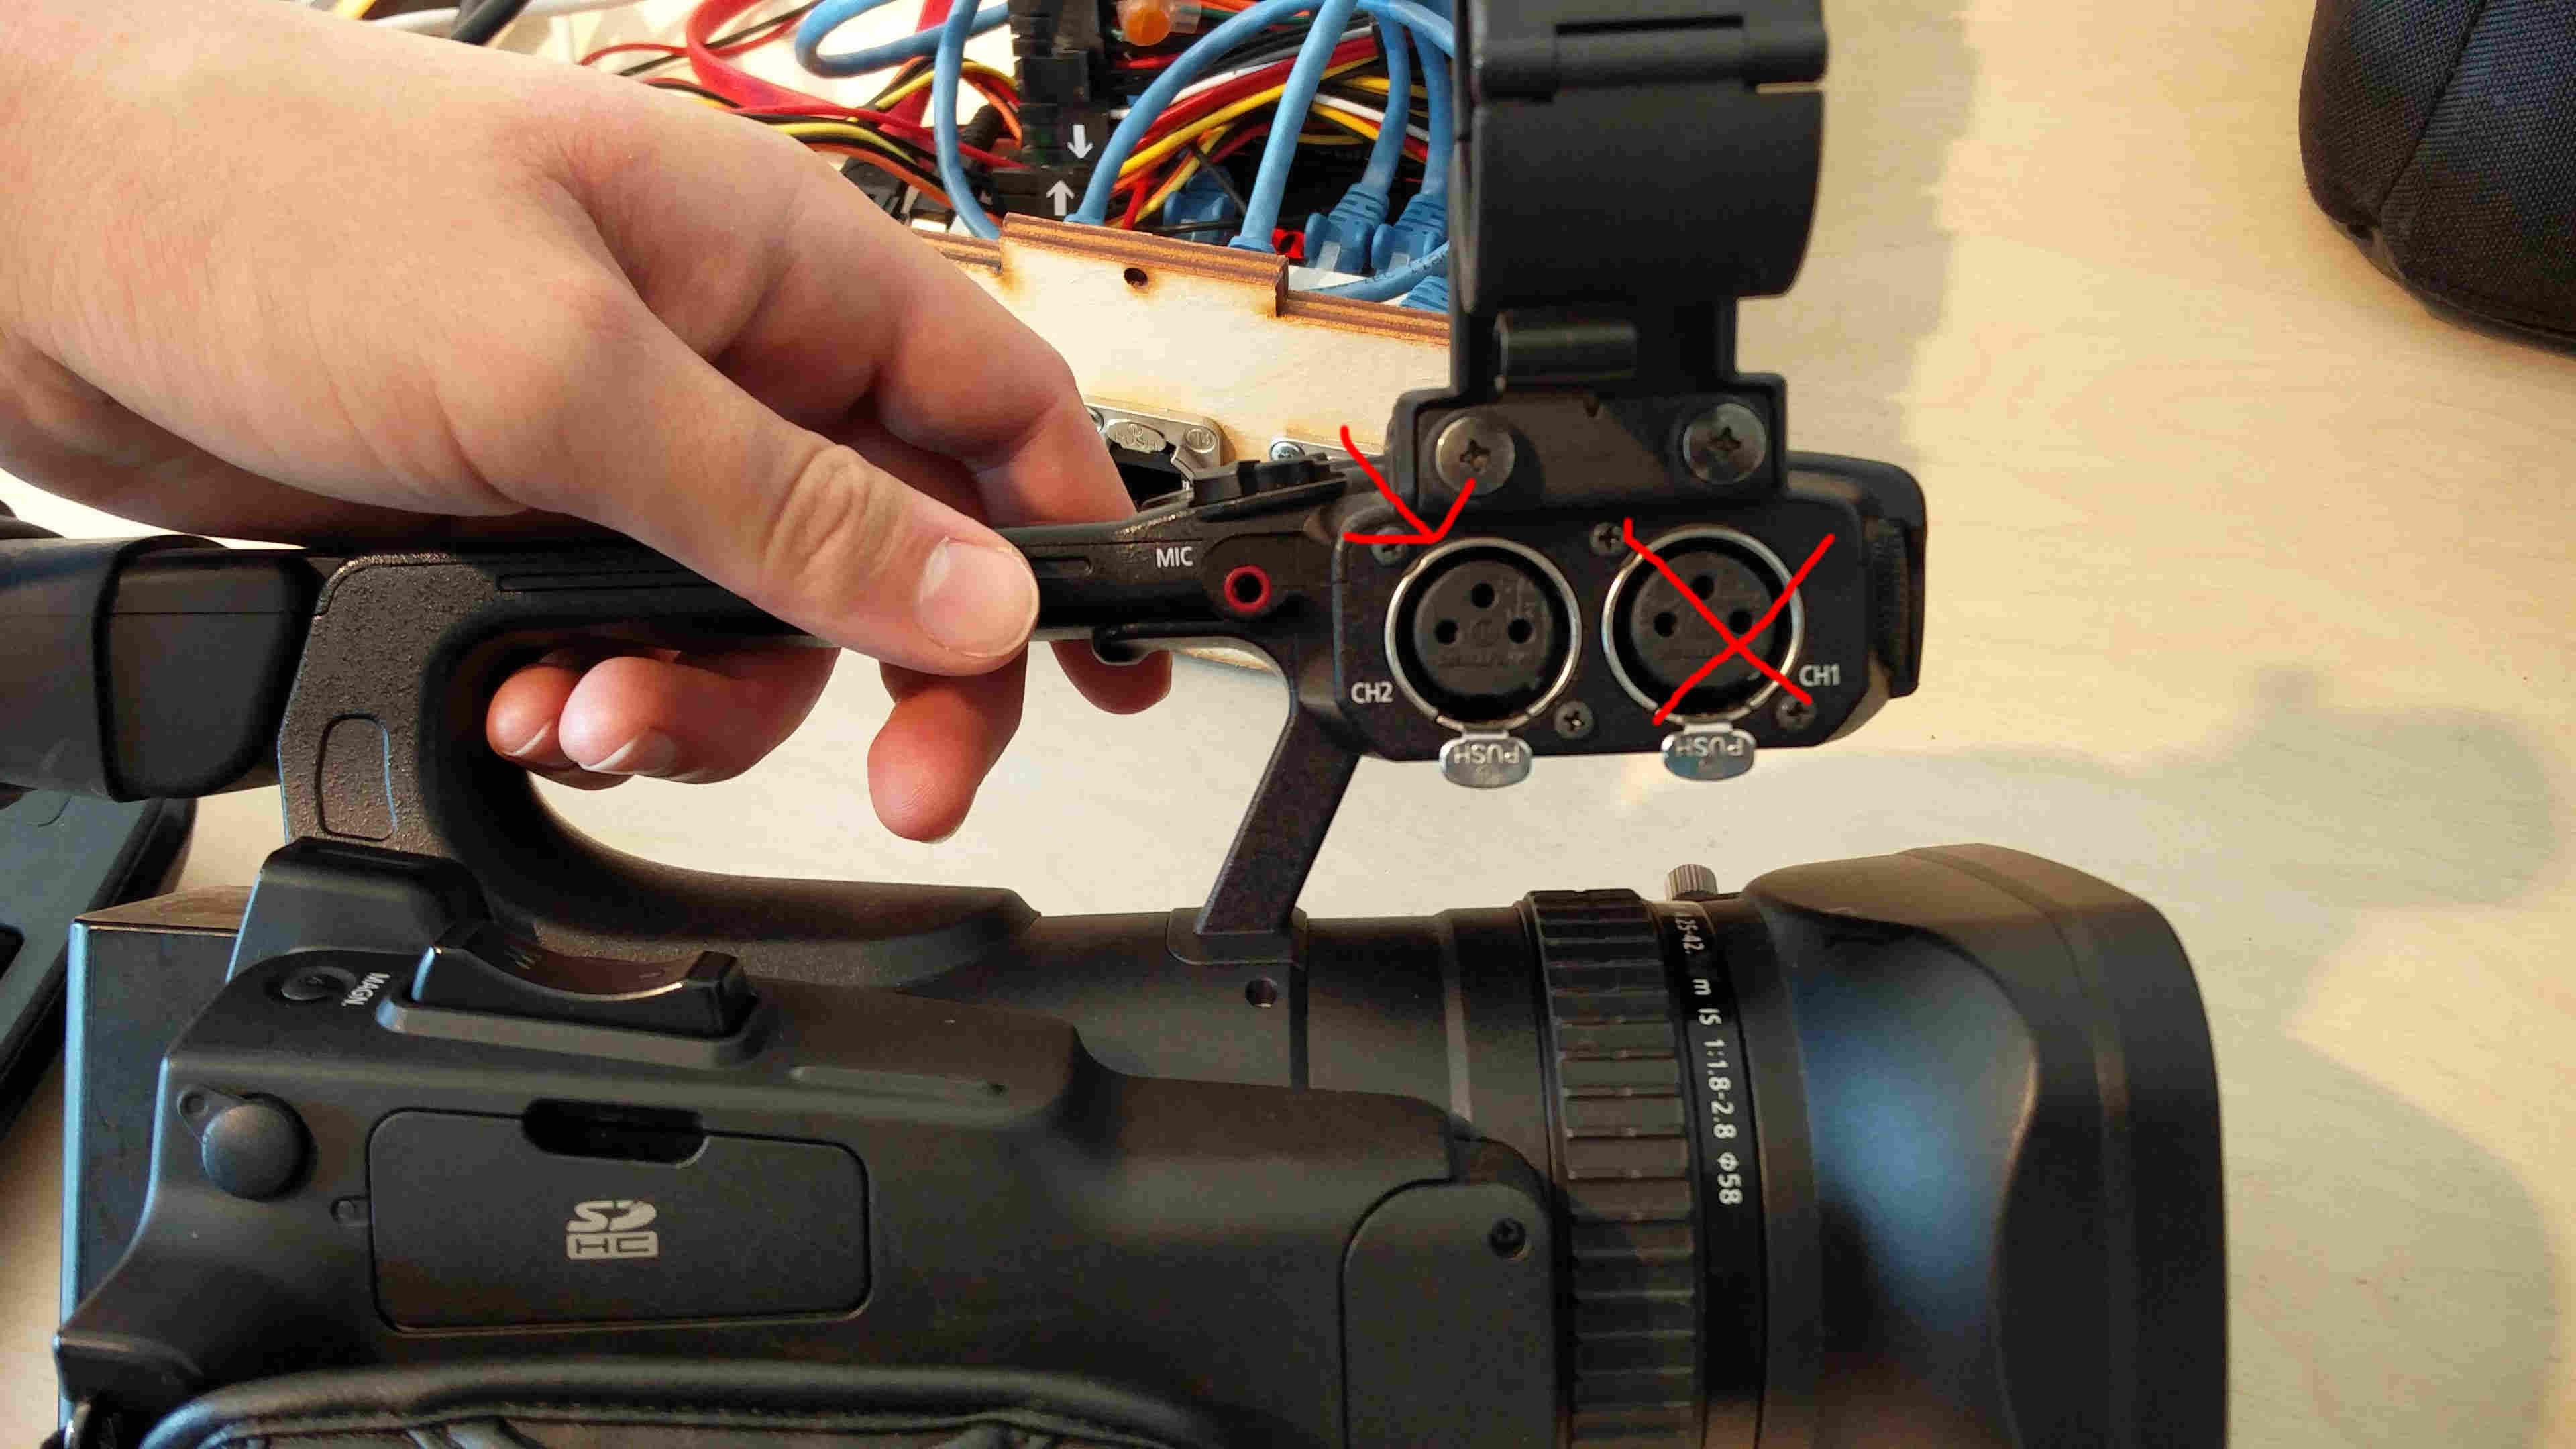
\includegraphics[width = 120mm]{Canon02.jpg}
\end{figure}

\subsubsection{Power on}
You can find the power button on the top of the left side of the camera (looking from behind).

\begin{figure}[H]
  \centering
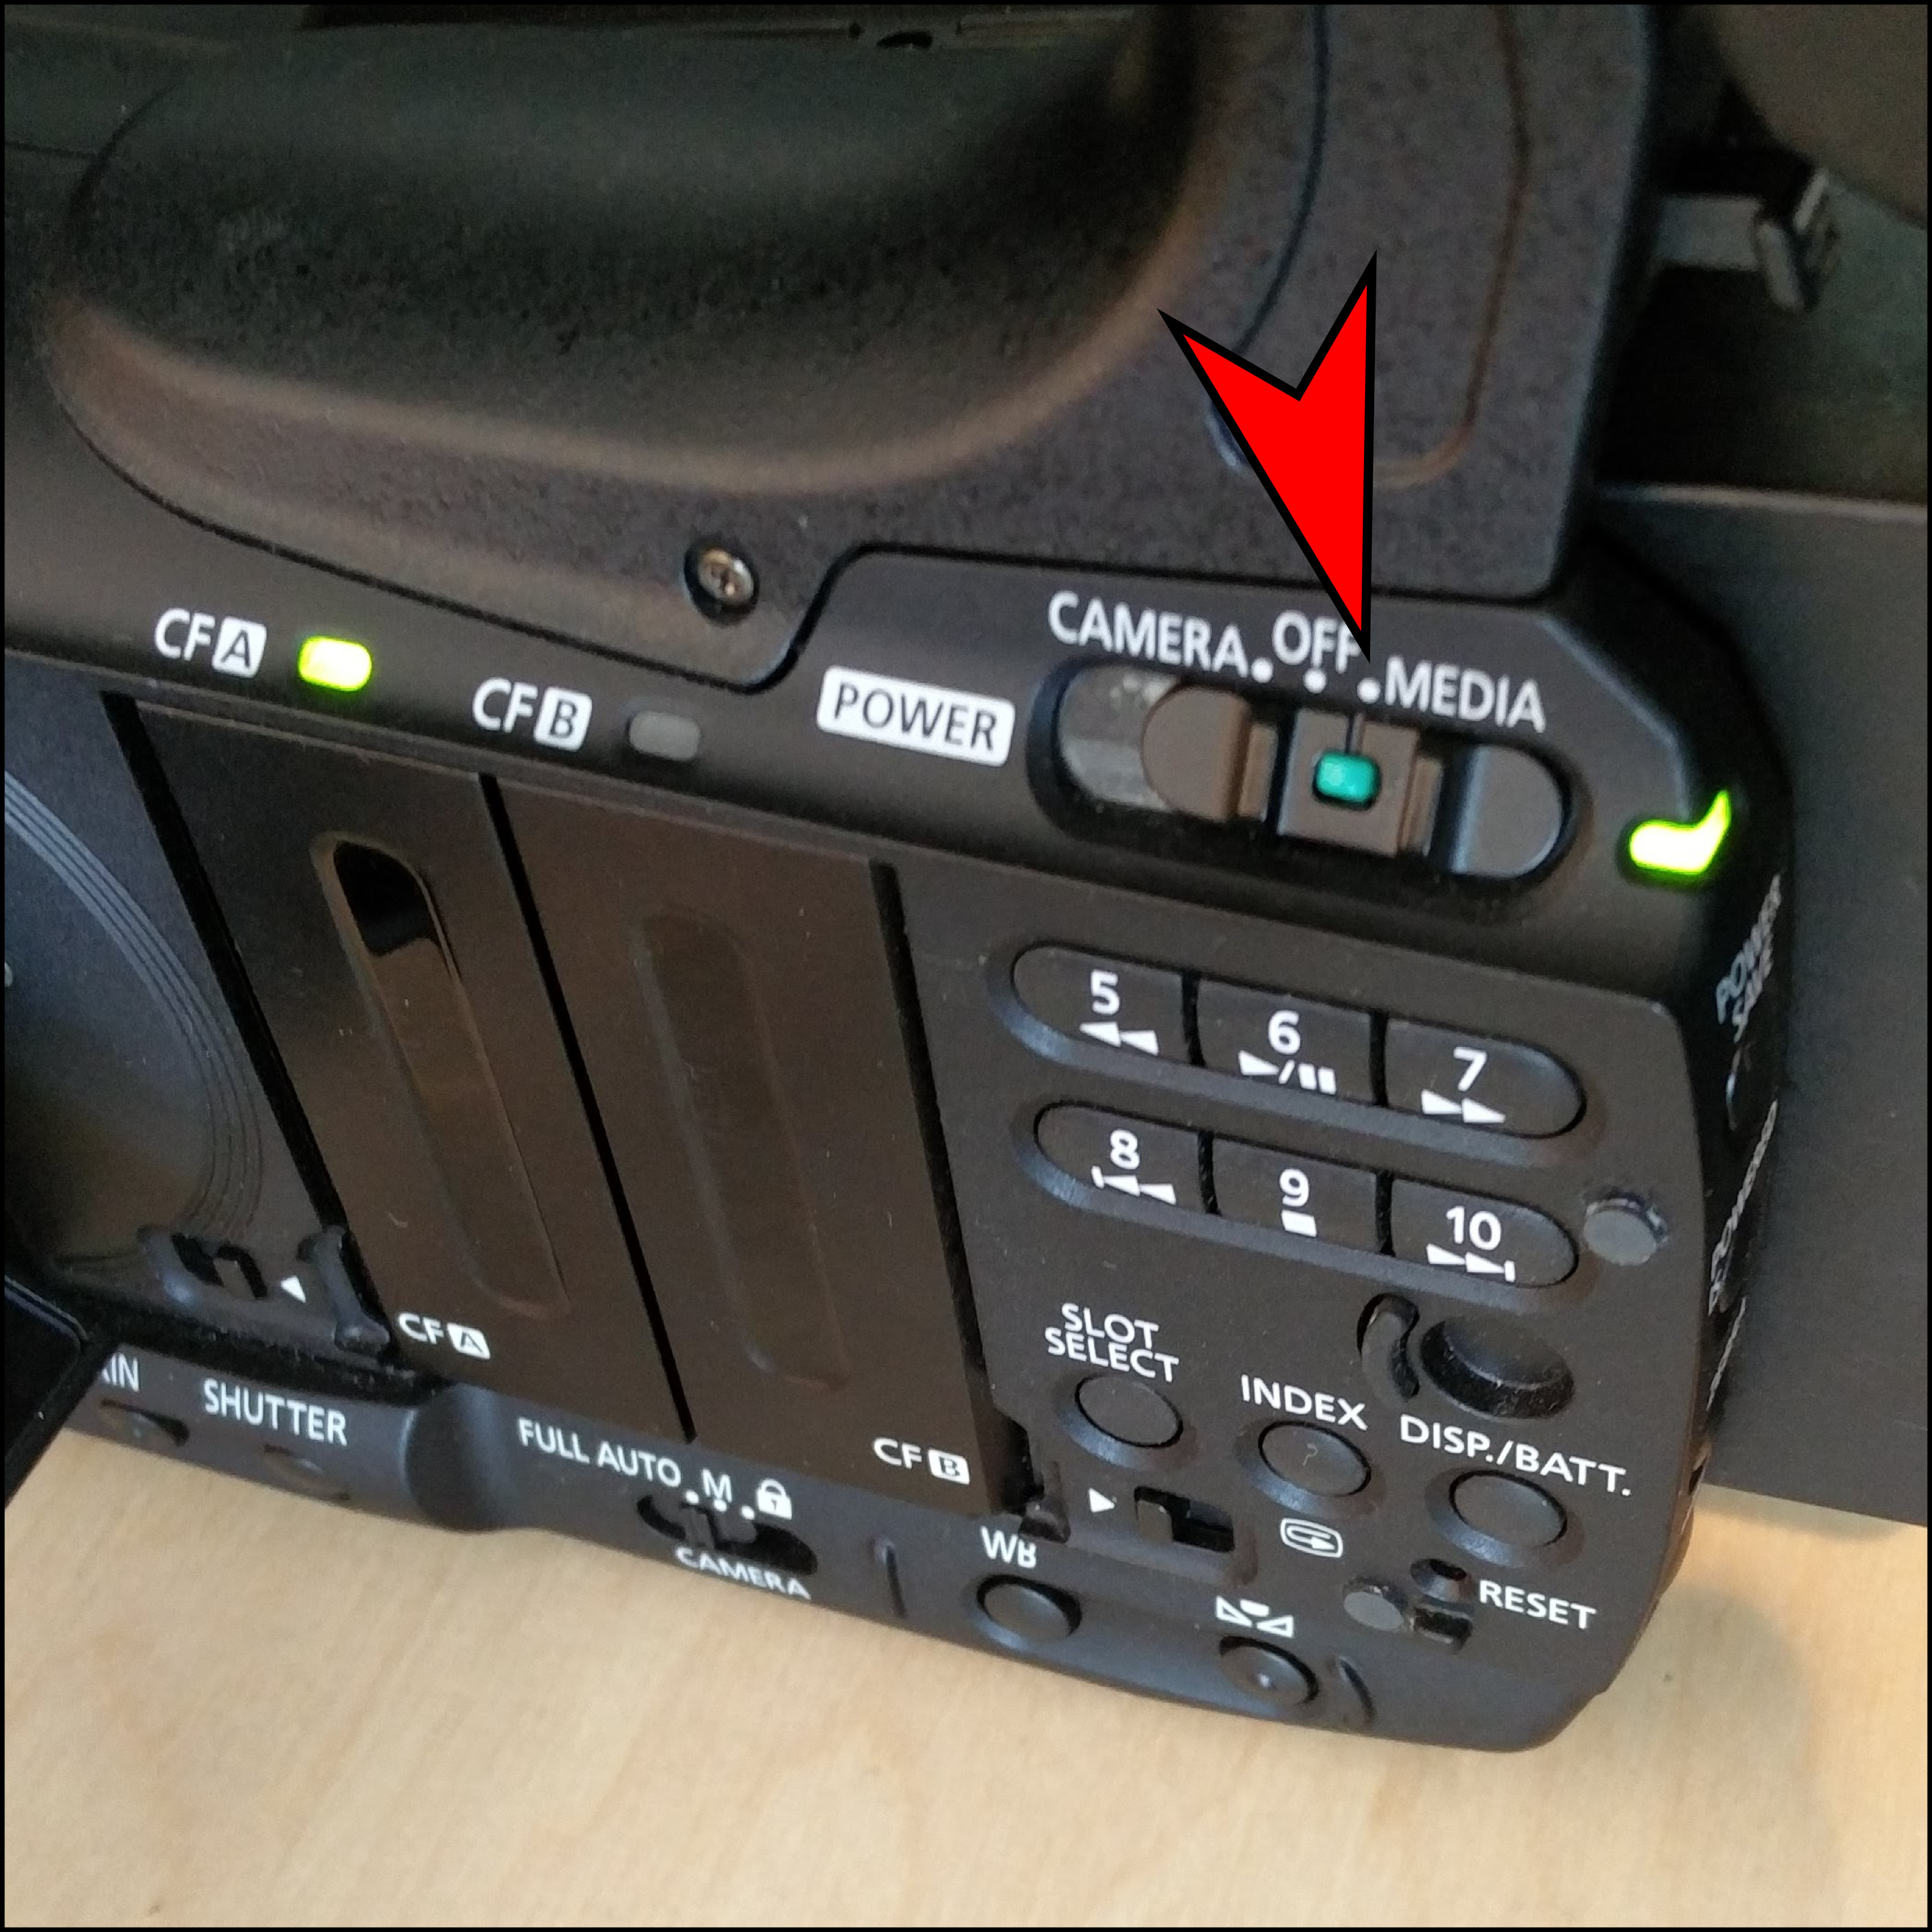
\includegraphics[width = 120mm]{Canon03.jpg}
\end{figure}

\subsubsection{Audio settings}
The audio settings can only be done through the hardware switches on the camera.
Make sure to set the switches to the correct positions, as these directly affect the availability of audio on the recordings and live streams. Wrong settings means no audio!
The position of the dials does not matter (those are for manual volume, we use automatic volume).
If unsure, verify with the image below.

\begin{tabular}{| l || l | l | l | l |}
Input & Top switch & Middle switch & Bottom switch & dial at top \\ \hline
CH1 & LEFT (A) & RIGHT (MIC 48V) & LEFT (INT) & anything \\
CH2 & LEFT (A) & LEFT (LINE) & RIGHT (EXT) & anything \\
\end{tabular}

\begin{figure}[H]
  \centering
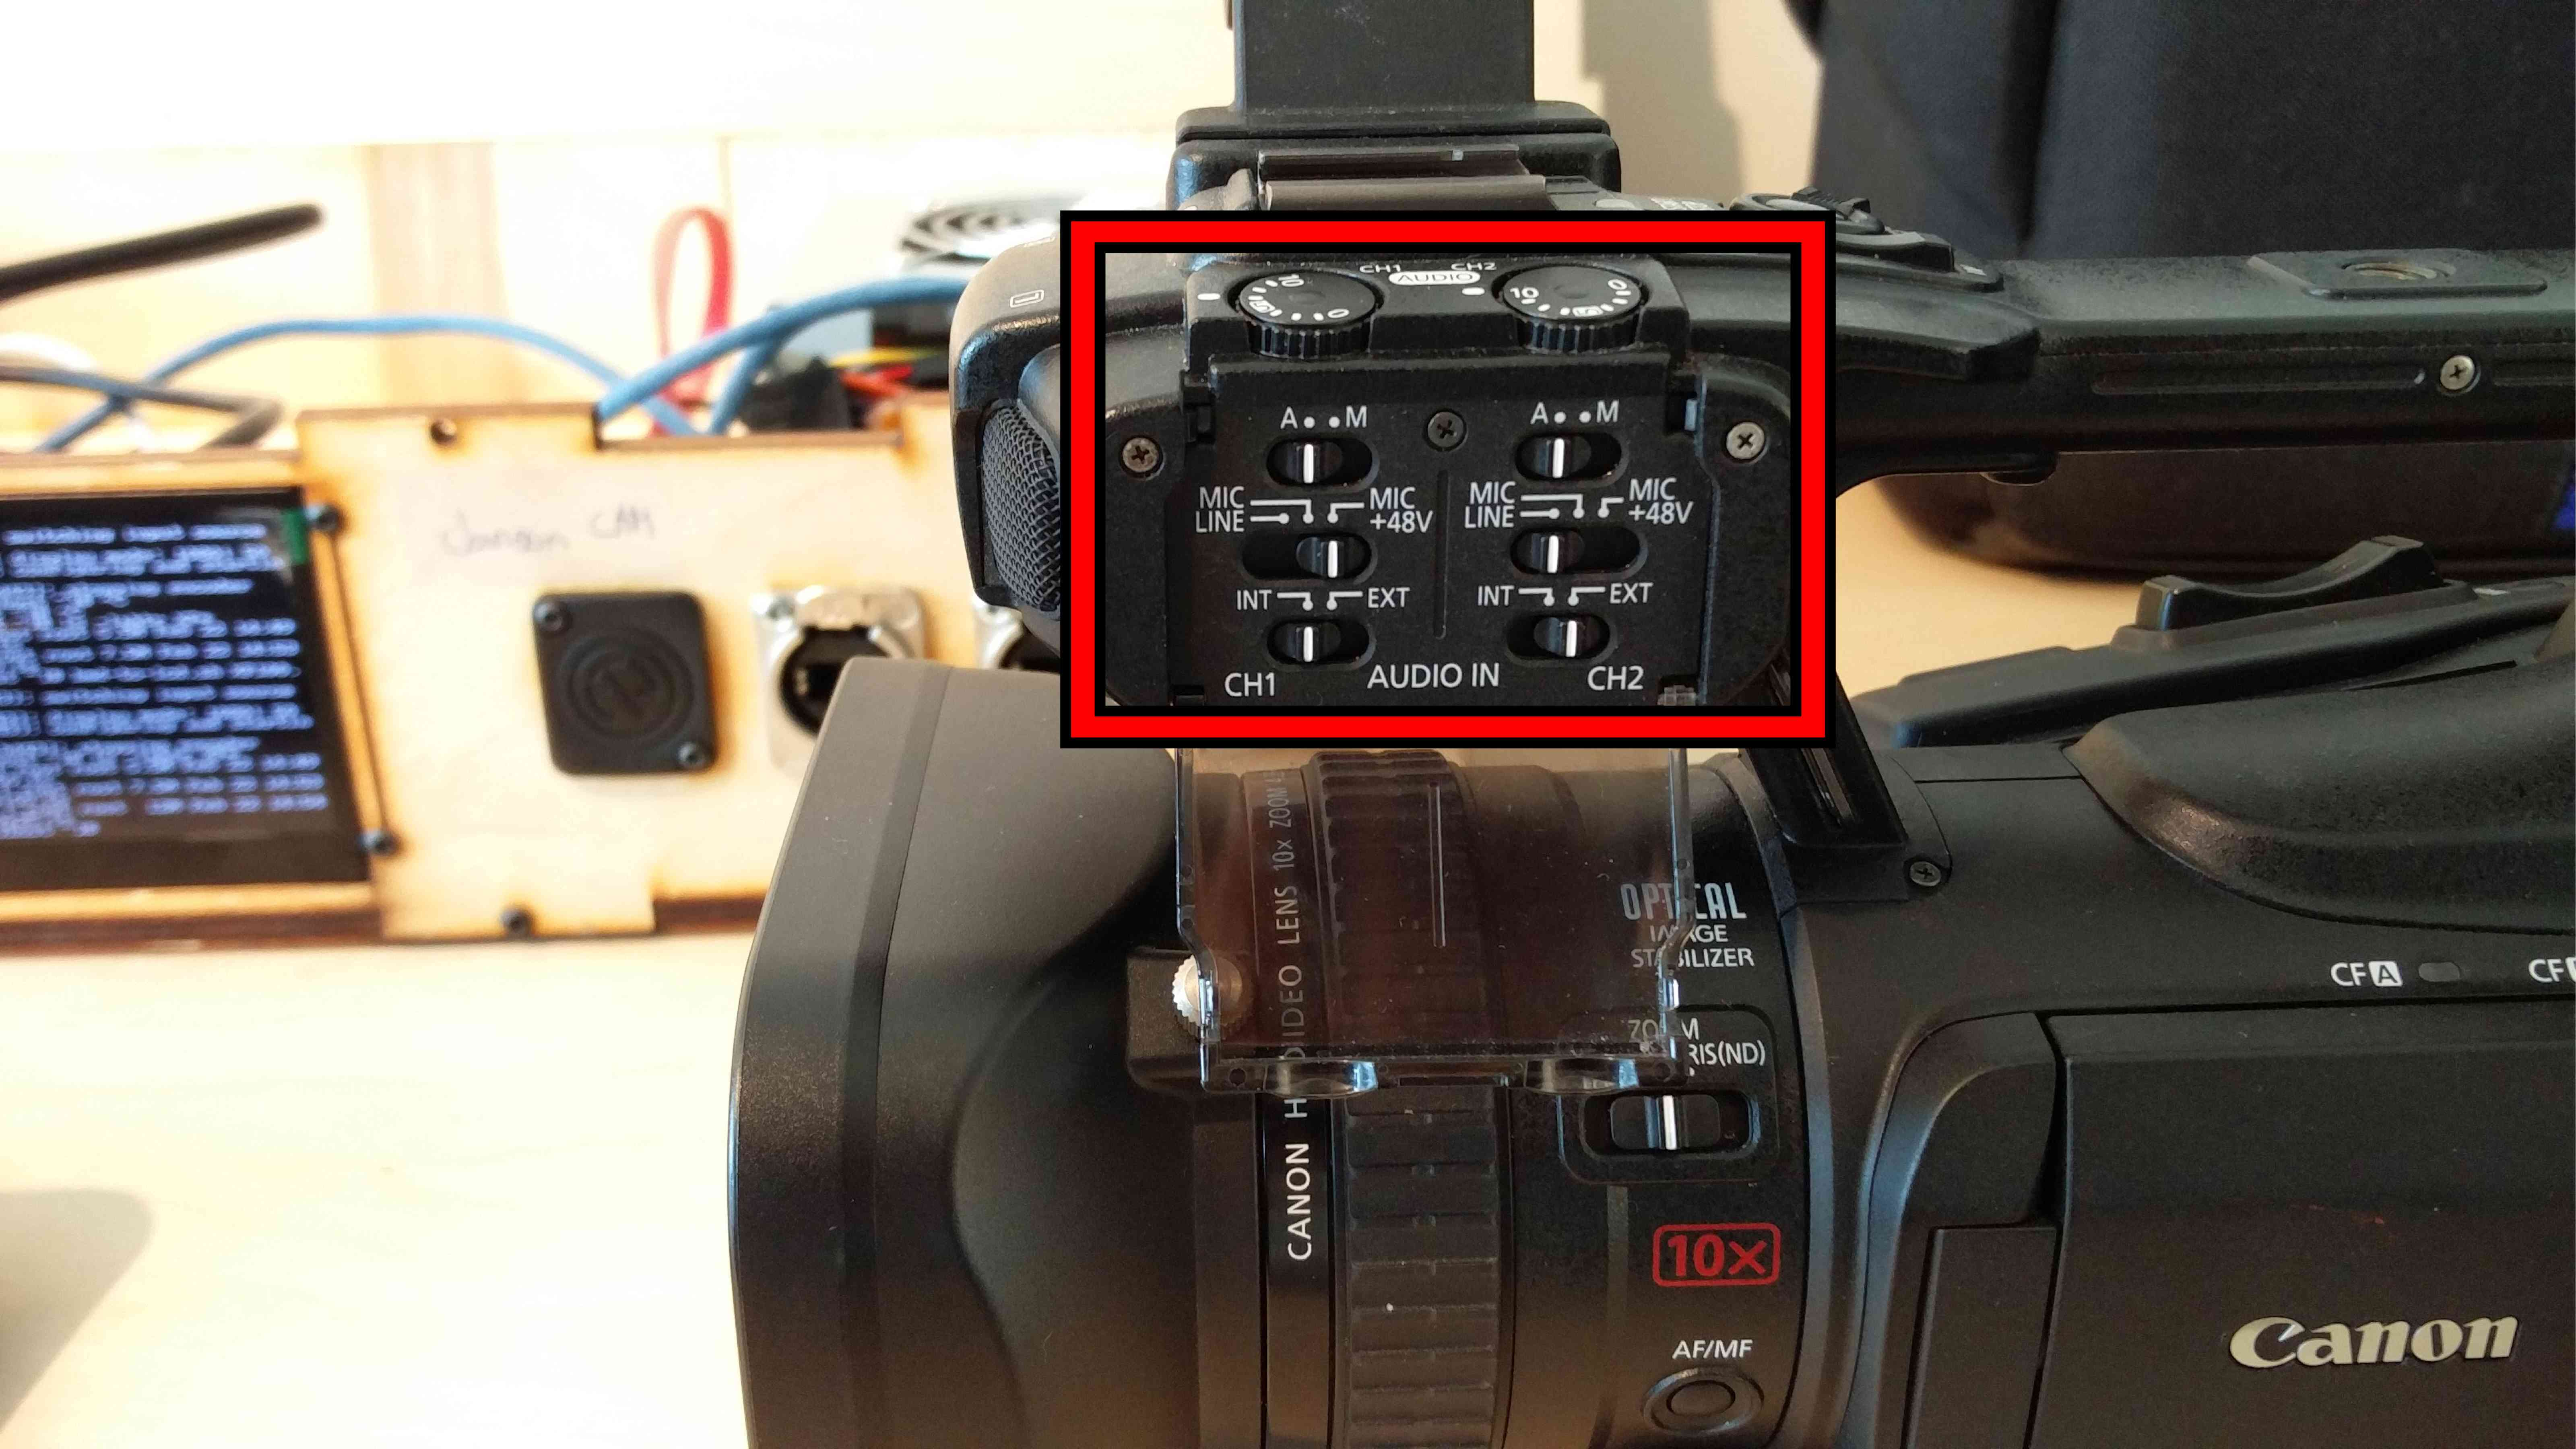
\includegraphics[width = 120mm]{Canon04.jpg}
\end{figure}

\subsubsection{Video settings}
The video settings will be done through the on-screen display.

Set up like this:

Menu $\rightarrow$ Last pictogram (wrench) $\rightarrow$ Bit Rate/Resolution $\rightarrow$ 1280x720 50Mbps

Menu $\rightarrow$ Last pictogram (wrench) $\rightarrow$ Frame Rate $\rightarrow$ 50P

\begin{figure}[H]
  \centering
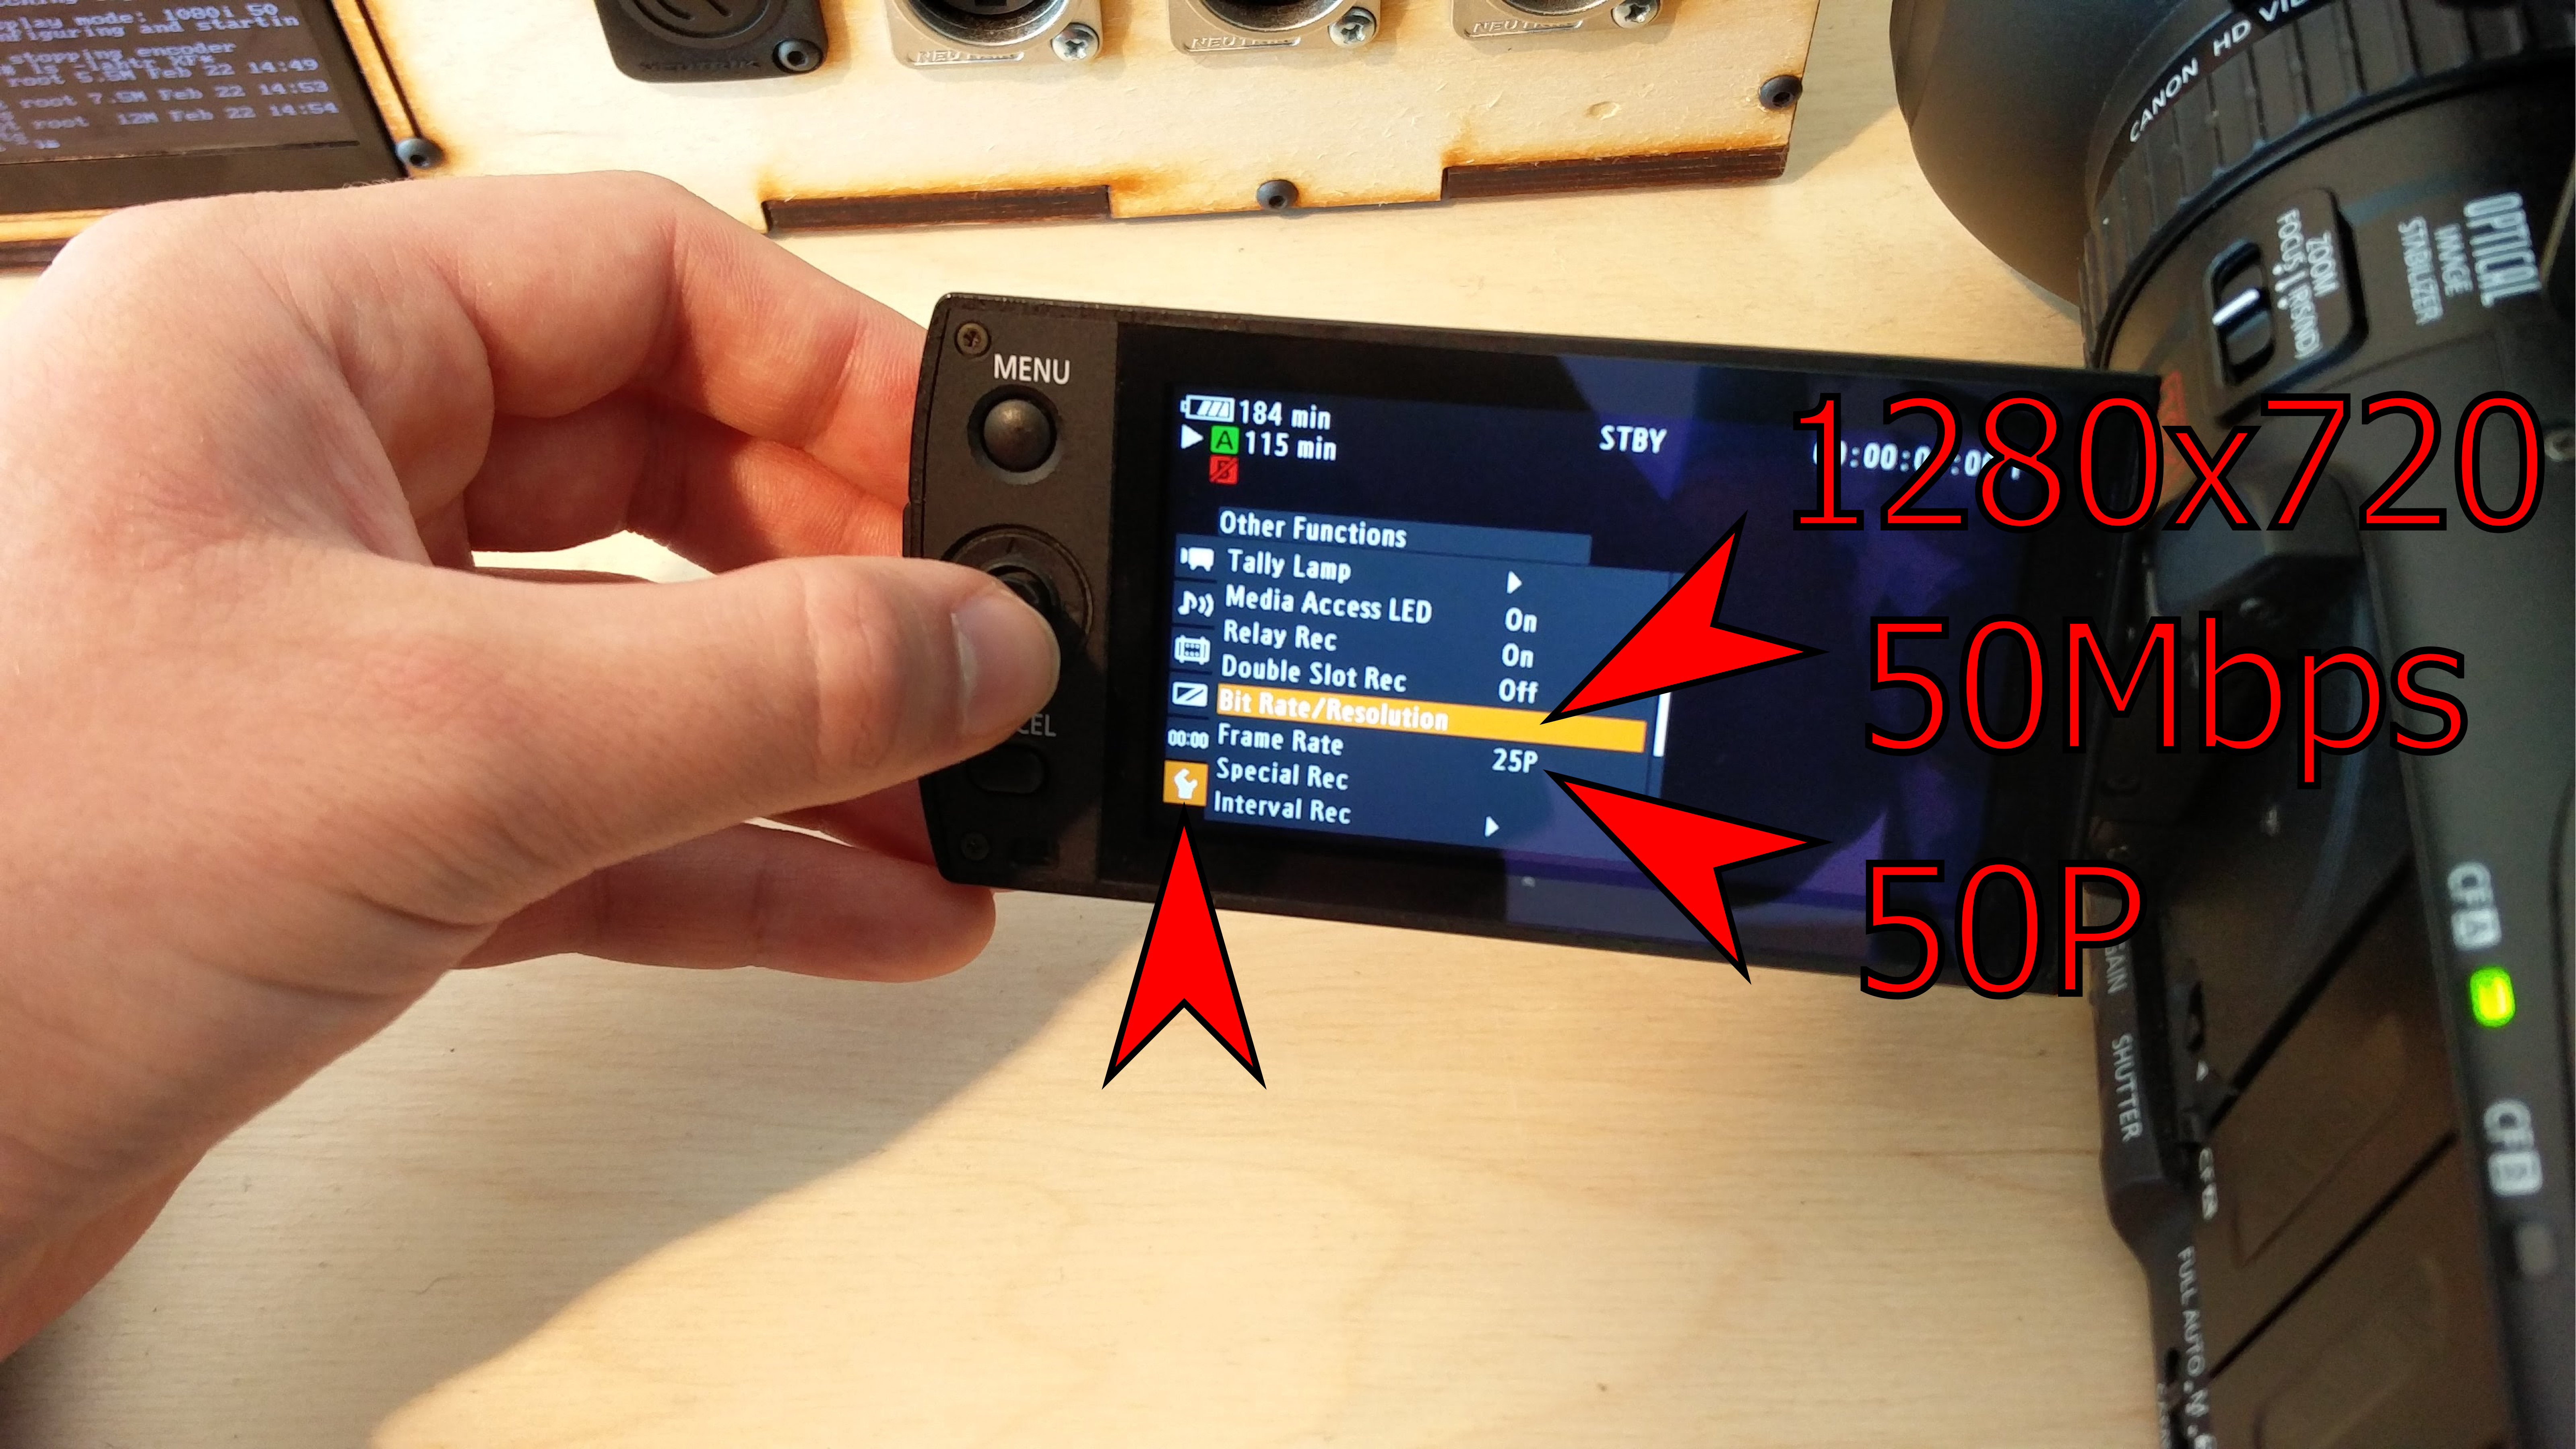
\includegraphics[width = 120mm]{Canon05.jpg}
\end{figure}

With this camera model, the on-screen display will show the configuration that is active during normal operation.
\begin{figure}[H]
  \centering
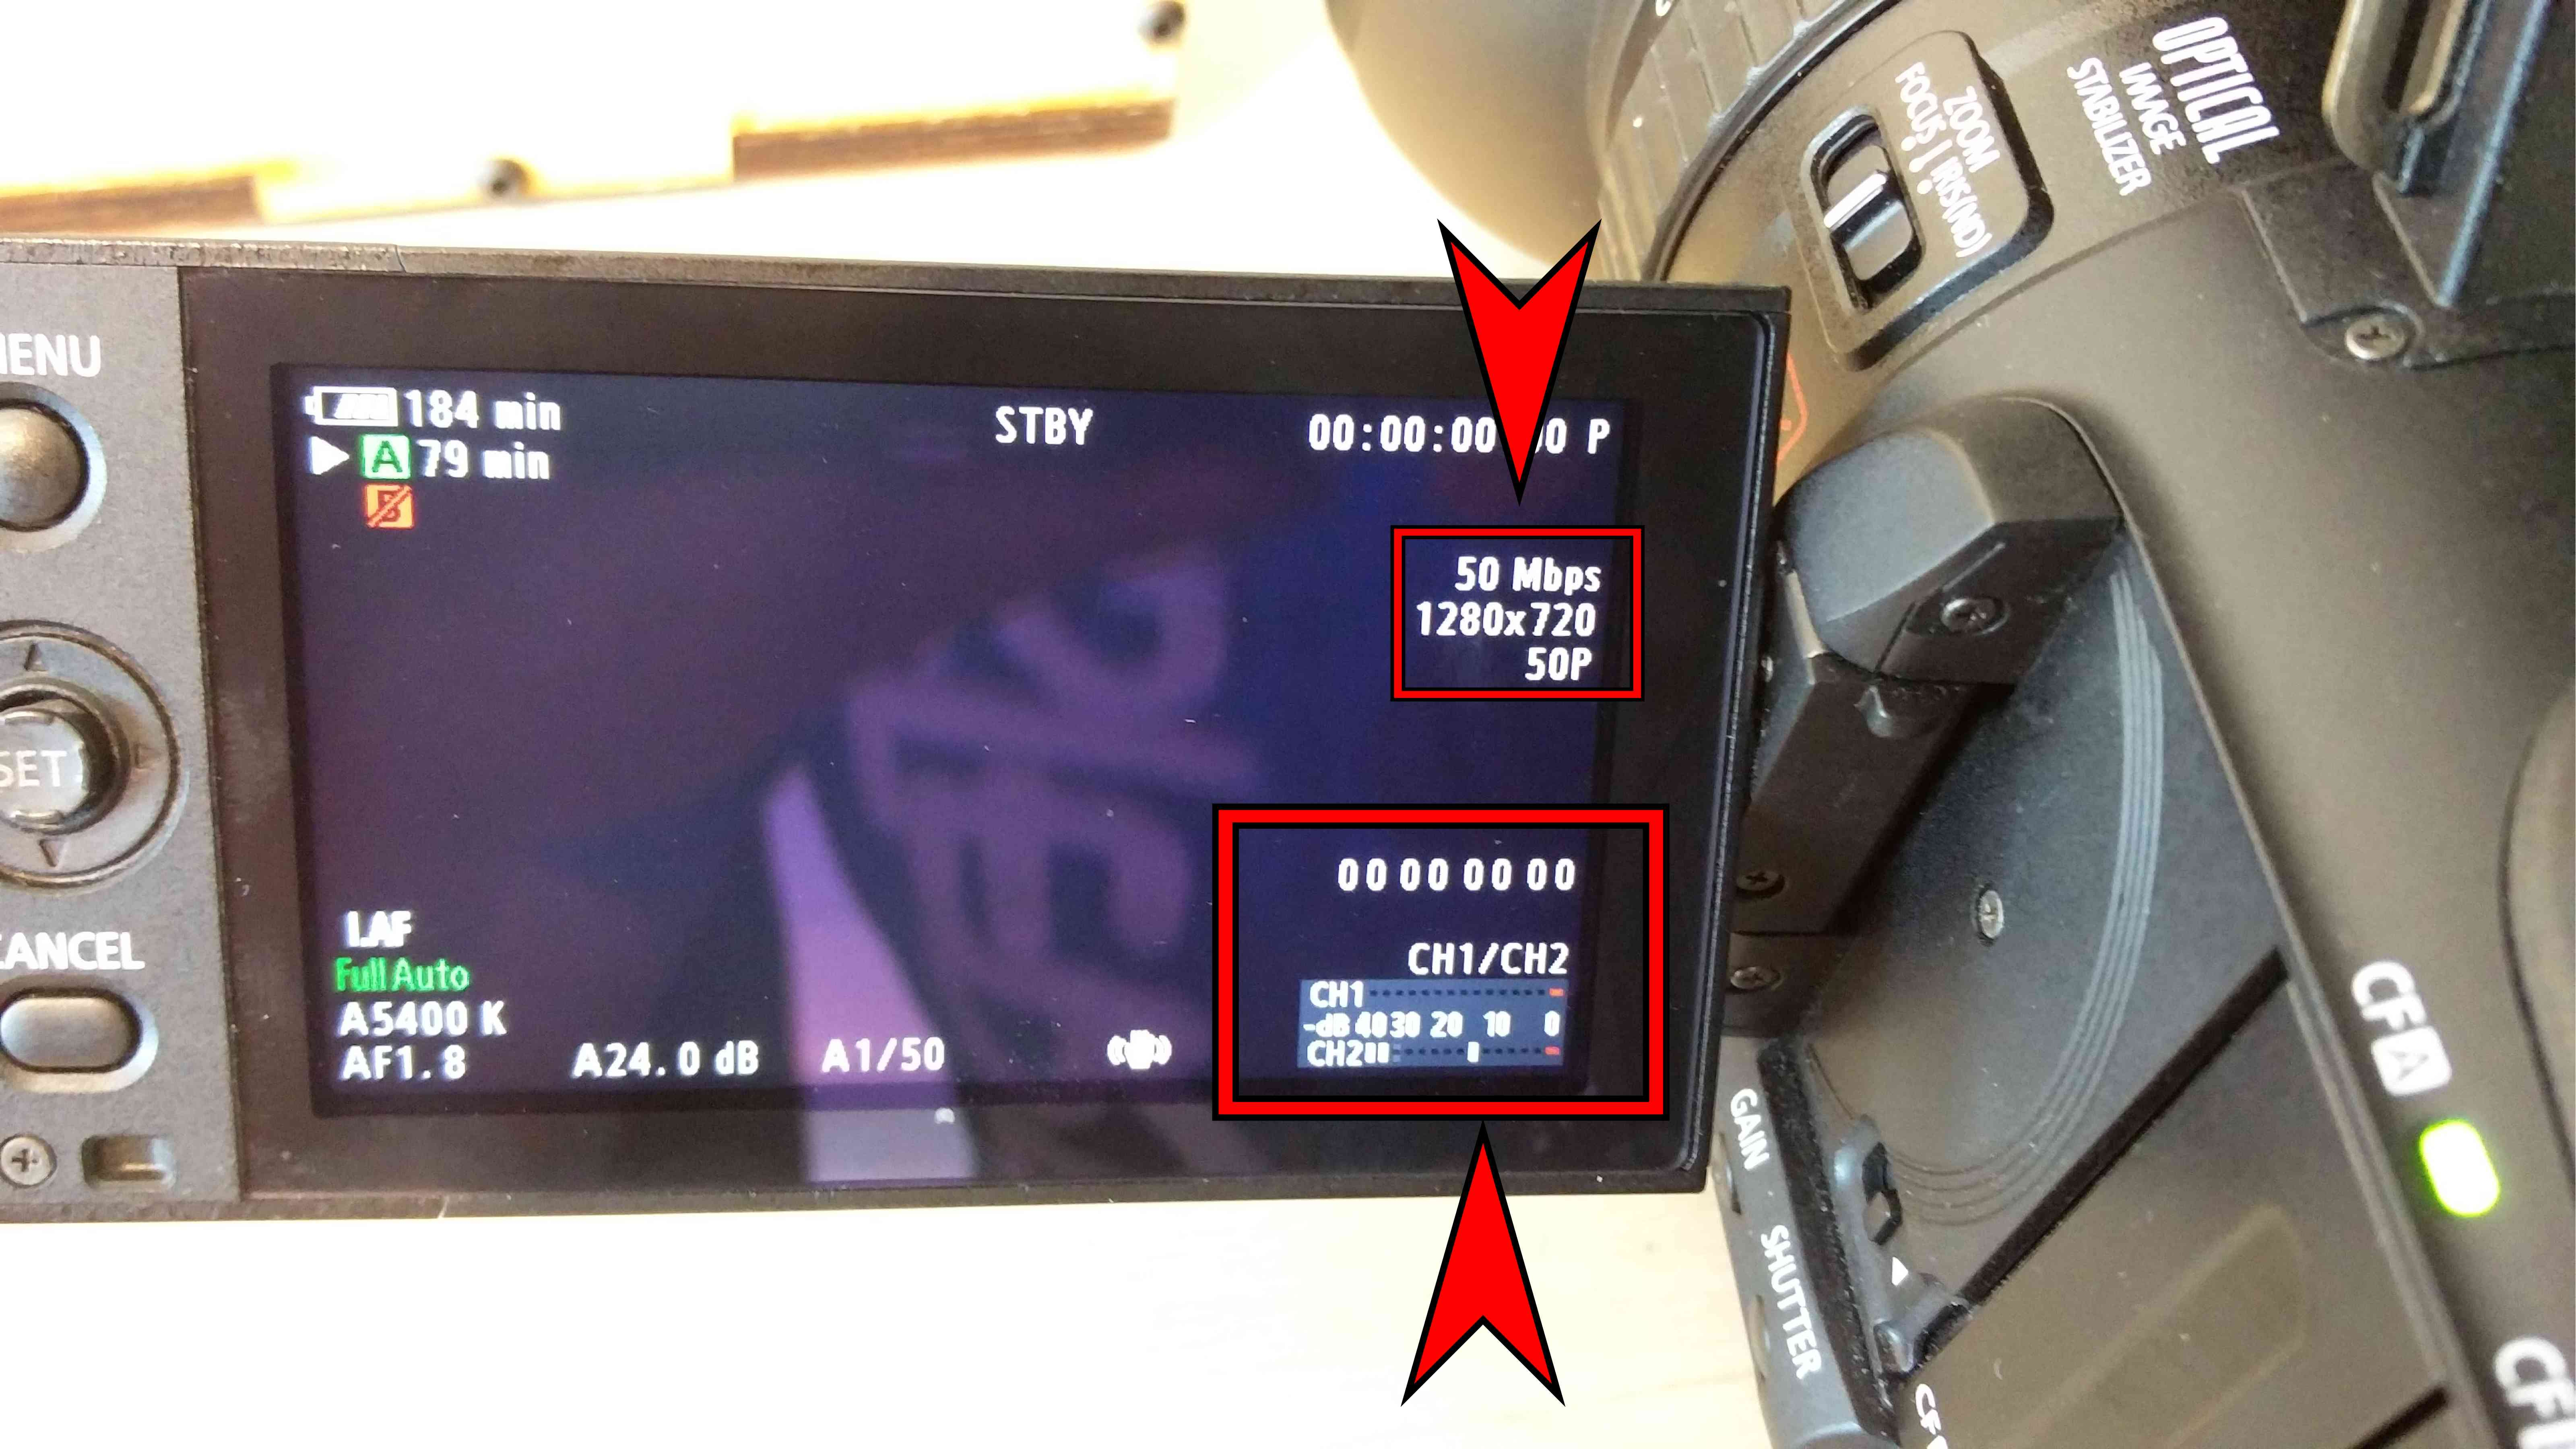
\includegraphics[width = 120mm]{Canon06.jpg}
\end{figure}

\subsubsection{Remove the lens cover}
Do not forget to remove the lens cover. Store it in the camera bag for safe keeping.

\begin{figure}[H]
  \centering
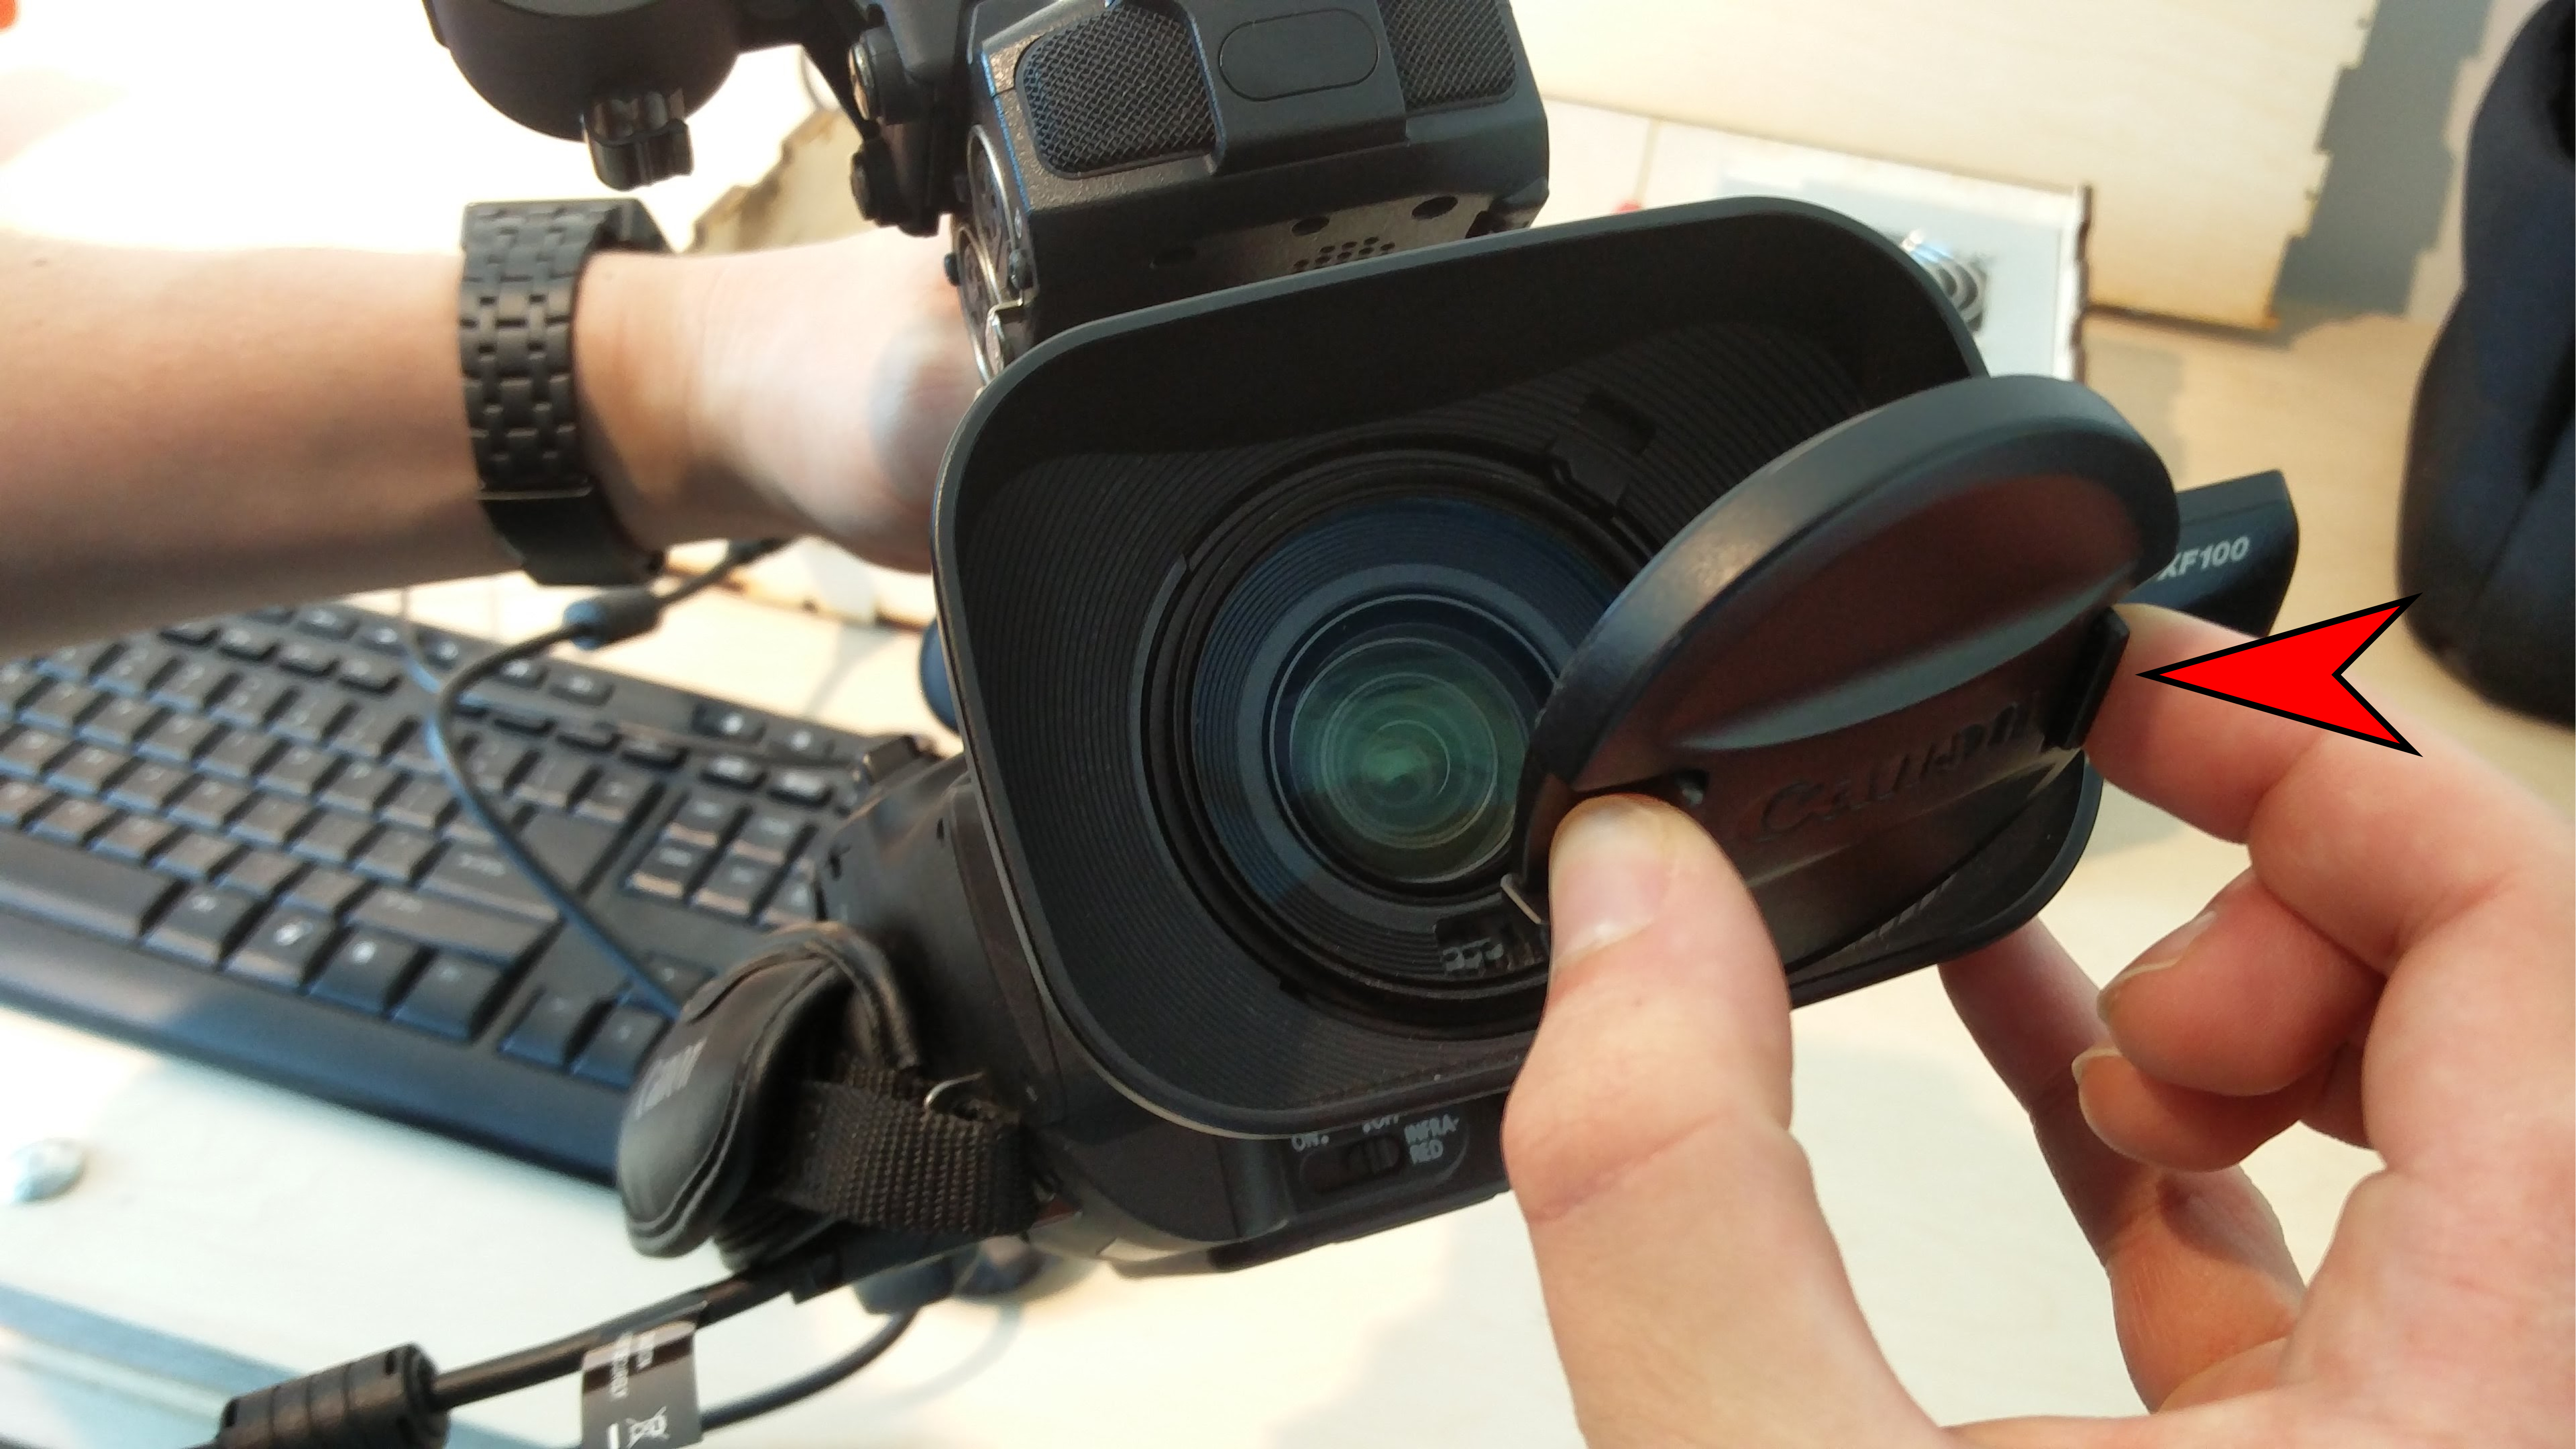
\includegraphics[width = 120mm]{Canon07.jpg}
\end{figure}

\subsubsection{Checklist}
Please check the following before leaving:
\begin{itemize}
  \item Does CH1 on the camera display spike when you tap the camera itself with your fingers?
  \item Does CH2 on the camera display spike when you tap the (powered on) wireless speaker microphone?
  \item Turn off the wireless speaker microphone before leaving to conserve battery power for during the day.
  \item Do both video boxes say mode 720p50 on the LCD display?
  \item Does the camera video box display the camera image on the LCD display?
\end{itemize}

If any of these do not work, re-check your connections and settings. Still no luck? Contract control!

\subsubsection{Contact control}
Please report that you've finished the room with your local control point.
They will let you know what rooms still need attention.

\section{During the event}
It is expected of the devroom video volunteers that they keep an eye on the following, in order of importance:
\begin{itemize}
  \item The wireless speaker mic is on during talks
  \item The wireless speaker mic is worn correctly
  \item The audio volume is not too low or too high (clipping is bad!)
  \item The camera is aimed at the speaker, \emph{not} the projection screen (the projection screen is captured separately!)
  \item None of the video equipment is stolen or tampered with
  \item The video box is turned on and has OK network status.
\end{itemize}
As you can see, the main task is ensuring audio quality. Video quality, will important, is only a secondary concern. A recording without video is still usable, but a recording without audio is completely useless.

Video team members will be both monitoring remotely as well as visiting rooms with problems. If you have questions, concerns or problems and there is no video team member nearby, contact them through the \texttt{\#fosdem-video} channel on the Freenode IRC service. If your video box shows issues on the LCD, most likely somebody is already on their way to you. When communicating with video team members, please mention the \emph{room number} as opposed to the devroom name. Devrooms move around, room numbers stay constant.

\end{document}
 
